\documentclass[professionalfont, handout, 12pt]{beamer} %, handout



%\usepackage{pxfonts}
%\usepackage{eulervm}

%\documentclass[sans,mathserif]{beamer}
%\usepackage{kerkis} % Kerkis roman and sans
%\usepackage{kmath}


%\documentclass[serif, professionalfont]{beamer} %
%\usepackage[T1]{fontenc} % Needed for Type1 Concrete
%\usepackage{concrete}


\usepackage{amsmath}
\usepackage{amsthm}
\usepackage{amsthm,amssymb,amsfonts,amsmath} 
\usepackage{proof}
\usepackage[mathscr]{eucal}
\usepackage{amssymb,mathtools}
\usepackage{xcolor}
\usepackage{mathrsfs}
\usepackage{enumerate}
\usepackage{comment}
\usepackage{pifont}
\usepackage{caption}

\usepackage{tikz}
\usetikzlibrary{shapes.geometric}
\usetikzlibrary{arrows}
\usetikzlibrary{shapes}
\usetikzlibrary{plotmarks}

\theoremstyle{plain}
\newtheorem{thm}{Theorem}
\newtheorem{remark}{Remark}
\newtheorem{cor}[thm]{Corollary}
 
\theoremstyle{definition}
\newtheorem{df}{Definition}
       
  
\usepackage{epsfig}
%\usepackage{amsmath}
%\usepackage{mathrsfs}
%\usepackage[all]{xy}  
%\usepackage{proof}    %%proof.style file
           

\newcommand{\tcb}[1]{\textcolor{blue}{#1}}
\newcommand{\tcr}[1]{\textcolor{red}{#1}}  
\newcommand{\tcc}[1]{\textcolor{cyan}{#1}}
\newcommand{\tcg}[1]{\textcolor{green}{#1}} 
\newcommand{\tcm}[1]{\textcolor{magenta}{#1}}      

\newcommand{\omt}{\mathop{\curlywedge}}
  
    
\newcommand{\Lra}{\: \Leftrightarrow \:}
\newcommand{\m}[1]{{\mathbf {#1} }}
%\newcommand{\m}[1]{{\mbox{\uppercase {\bf {#1}}}}}
%\newcommand{\N}[1]{{{ \m N_{#1}}}}
\newcommand{\Rl}{ {\mbox{$\mathcal{RL}  $}}}
\newcommand{\Rlc}{ {\mbox{$\mathcal{RL}^C  $}}}
\newcommand{\Ra}{{ \:\; \Rightarrow \:\; }}
%\newcommand{\Ra}{{\mbox{$ \: \Rightarrow \: $}}}
\newcommand{\Rar}{{ \: \Rightarrow \: }}
\newcommand{\La}{{\mbox{$ \: \Leftarrow \: $}}}
\newcommand{\ra}{\rightarrow}
\newcommand{\la}{\leftarrow}
\newcommand{\lra}{\leftrightarrow}
\newcommand{\fa}{\: \forall}
\newcommand{\lan}{(}
\newcommand{\ran}{)}
\newcommand{\rl}{{residuated lattice }}
\newcommand{\rls}{{residuated lattices }}
\newcommand{\T}{\top}
\newcommand{\jn}{\vee}
\newcommand{\mt}{\wedge}
\newcommand{\ror}{\: $ or $ \:}
\newcommand{\rand}{\: $ and $ \:}
\newcommand{\Tg}{\lan \T \ran}
\newcommand{\set}[2]{{\mbox{$ \{ #1 \: | \: #2 \}  $}}}
\newcommand{\ex}{\exists}
\newcommand{\eq}{\approx}
\newcommand{\eqv}{\cong}
\newcommand{\sbs}{\subseteq}
\newcommand{\sps}{\supseteq}
\newcommand{\vr}{{\mbox{$\mathcal{V}$}}}
\newcommand{\Vr}{{\mbox{$ \mathcal{V} \: $ }}}
\newcommand{\vrg}[1]{{\mbox{ $ \mathcal{V}  (\m #1) $}}}
\newcommand{\vs}{\emptyset}
\newcommand{\cov}{\prec}
\newcommand{\rd}{{/}}
\newcommand{\ld}{{\setminus}}
%\newcommand{\qed}{\hfill$\bullet$}
\newcommand{\ol}{\overline}
%\newcommand{\ua}{\hspace{.04in} \uparrow \hspace{-.04in}}
\newcommand{\ua}{\mathop{\uparrow}}
\newcommand{\da}{\hspace{.01in} \downarrow \hspace{-.01in}}
\newcommand{\dm}{\stackrel{\cdot}{-}}
\newcommand{\md}{\stackrel{-}{\cdot}}
\newcommand{\bra}{{\bf \ra}}
\newcommand{\blra}{{\bf \lra}}
\newcommand{\ban}{{\bf \&}}
\newcommand{\bor}{{\bf \nabla}}
\newcommand{\bmt}{{\bf \mt}}
\newcommand{\bjn}{{\bf \jn}}
\newcommand{\bneg}{{\bf \neg}}
\newcommand{\bbot}{{\bf \bot}}
\newcommand{\btop}{{\bf \top}}
\newcommand{\entails}{\vdash}
\newcommand{\TM}{{\mbox{{Turing Machine }}}}
\newcommand{\TMs}{{Turing Machines }}
\newcommand{\MM}{{Minskii Machine }}
\newcommand{\RA}{\Ra}
\newcommand{\rla}{{relation algebra }}
\newcommand{\rlas}{{relation algebras }}
\newcommand{\cv}{ ^{ \cup } }
\newcommand{\cg}{{\rm Cg}}                          %Petar
\newcommand{\var}[1]{{\uppercase \mathcal{{#1}}}}      %Petar
\newcommand{\Lg}{{\mbox{$\mathcal{LG} $}}}             %Partick
\newcommand{\Lgm}{{\mbox{$\mathcal{LG}^- $}}}          %Partick
\newcommand{\phibar}{{\mbox{$\ol \phi\ $}}}         %Partick
\newcommand{\vrm}{{\mbox{$\mathcal{V}^- $}}}           %Partick
\newcommand{\Ya}{\Rightarrow}
\newcommand{\bs}{\boldsymbol}
\newcommand{\cleq}{\preceq}
\newcommand{\hra}{\rightharpoonup}
\renewcommand{\ln}{\mathord{\sim}}
\newcommand{\rn}{\mathord{-}}
\newcommand{\lrh}{\mathop{\leftrightarrow}}
\providecommand{\semsb}{\ensuremath{\mathscr{M}}}
\providecommand{\sem}[1]{\ensuremath{\semsb (#1)}} 
\newcommand{\alhack}{\\[-\normalbaselineskip]\tag*{\qedhere}}
\providecommand{\psetsb}{\ensuremath{\mathscr{P}}}
\providecommand{\pset}[1]{\ensuremath{\psetsb (#1)}} 
\providecommand{\pfin}[1]{\ensuremath{\psetsb_{\text{fin}}(#1)}}

\newcommand{\co}{\mathsf} %fontshape for class operators
\newcommand{\cl}{\mathcal} %fontshape for general classes
\newcommand{\RL}{\va{RL}}
\DeclareMathOperator{\Mod}{Mod}
\newcommand{\bl}{\boldsymbol{\Lambda}}

% Macros for FL
\newcommand{\al}{\alpha}
\newcommand{\sig}{\Sigma}
\newcommand{\lam}{\Lambda}
\newcommand{\gam}{\Gamma}
\newcommand{\del}{\Delta}
\newcommand{\im}{\rightarrow}
\newcommand{\ya}{\rightarrow}
\newcommand{\naraba}{\rightarrow}
\newcommand{\To}{\vdash}
%\newcommand{\lan}{\left(} %not \la
%\newcommand{\ran}{\right)} %not \ra
%\newcommand{\Ya}{\Rightarrow}
\newcommand{\noi}{\noindent}
%\newcommand{\preast}{{\preceq}^{\ast}}
%\newcommand{\prestar}{{\preceq}^{\star}}
\newcommand{\epsi}{\varepsilon}
\newcommand{\e}{\varepsilon}

\newcommand{\p}{\vskip 12pt}
\newcommand{\q}{\vskip 6pt}


\newcommand{\btl}{\lhd}%{\triangleleft}{\blacktriangleleft}
\newcommand{\btr}{\rhd}%{\triangleright}{\blacktriangleright} 
\newcommand{\eb}[1]{\emph{\textcolor{blue}{#1}}}       
\newcommand{\cb}[1]{\textcolor{blue}{#1}} 
\newcommand{\cred}[1]{\textcolor{red}{#1}}        
\newcommand{\ldd}{\mathbin{\bbslash}}
\newcommand{\rdd}{\mathbin{\sslash}}  
\newcommand{\raa}{\mathbin{\leadsto}}    
\newcommand{\RarN}{{\sqsubseteq}}  %{{\mathrel{N}}} 
\newcommand{\RaN}{\mathnormal{\RarN}}

\newcommand{\va}{\mathsf} %fontshape for specific varieties  
\newcommand{\cnv}{u}

\renewcommand{\And}{\text{ \sf and }} %already exists in LaTeX
\newcommand{\Or}{\text{ \sf or }}
\newcommand{\AND}{\text{\sf{AND }}}
\newcommand{\bcdw}{\mbox{\boldmath{$\,\cdot\,$}}}


\renewcommand{\and}{\text{ \sf and }}
\newcommand{\orc}{\text{ \sf or }}
\newcommand{\orb}{\ \overline{\mbox{\sf or}}\ }
\newcommand{\Implies}{\Longrightarrow}
\providecommand{\undsc}{\underline{\phantom{x}}}

\newcommand{\gal}[1]{#1^+}

\newcommand{\force}{\vdash}
\def\hh{\ |\ }
\newcommand{\FL}{\mbox{$\mbox{\bf FL}$}}

\newcommand{\ls}{\setbox0\hbox{$-$}
\mathbin{\hbox{$-$\kern-\wd0\raise2\dp0\hbox{$\cdot$}\kern.3\wd0\lower2\dp0\hbox
{$\cdot$}}}}
\newcommand{\rs}{\setbox0\hbox{$-$}
\mathbin{\hbox{$-$\kern-\wd0\lower2\dp0\hbox{$\cdot$}\kern.3\wd0\raise2\dp0\hbox
{$\cdot$}}}}

\newcommand{\rdo}{\mathop{\mbox{$\bigcirc \! \! \! \! \! \rdd \, $}}}
\newcommand{\ldo}{\mathop{\mbox{$\bigcirc \! \! \! \! \! \ldd \, $}}}

\newcommand{\cmark}{\ding{51}}
\newcommand{\xmark}{\ding{55}}

%Lattices 
\providecommand{\MEET}{\ensuremath{\bigwedge}}
\providecommand{\Meet}{\ensuremath{\textstyle\bigwedge\limits}}
\providecommand{\Join}{\ensuremath{\bigvee}}
\providecommand{\meet}{\ensuremath{\wedge}}
\providecommand{\join}{\ensuremath{\vee}}

%Set Theory
\providecommand{\card}[1]{\ensuremath{\left\lvert#1\right\rvert}}
\providecommand{\intersect}{\ensuremath{\cap}}
\providecommand{\Intersect}{\ensuremath{\bigcap}}
\providecommand{\union}{\ensuremath{\cup}}
\providecommand{\UNION}{\ensuremath{\bigcup}}
\providecommand{\Union}{\ensuremath{\textstyle\bigcup\limits}}
%Logic
\providecommand{\iff}{\ensuremath{\Leftrightarrow}}
\providecommand{\implies}{\ensuremath{\Rightarrow}}

%Algebra
\providecommand{\normal}{\ensuremath{\unlhd}}
\providecommand{\embed}{\ensuremath{\hookrightarrow}}%inclusion map
\providecommand{\gen}[1]{\ensuremath{\left<#1\right>}}%Group generated by #1
\providecommand{\idx}[2]{\ensuremath{\left[#1:#2\right]}}%index of #2 in #1
\providecommand{\order}[1]{\ensuremath{\left\lvert#1\right\rvert}}

%Commonly used Sets
\providecommand{\C}{\ensuremath{\mathbb{C}}}%complex
\providecommand{\N}{\ensuremath{\mathbb{N}}}%natural
\providecommand{\Q}{\ensuremath{\mathbb{Q}}}%rationals
\providecommand{\R}{\ensuremath{\mathbb{R}}}%reals
\providecommand{\Z}{\ensuremath{\mathbb{Z}}}%integers
\providecommand{\Zpos}{\ensuremath{\mathbb{Z}^{+}}}%positive integers

%functions
\providecommand{\restrictedto}{\ensuremath{\downharpoonright}}

%Analysis and lineal algebra
\providecommand{\norm}[1]{\ensuremath{\left\lVert#1\right\rVert}}
\providecommand{\vect}{\ensuremath{\vec}}

%Miscellaneous
\providecommand{\abs}[1]{\ensuremath{\left\lvert#1\right\rvert}}
\providecommand{\define}{\ensuremath{\stackrel{\text{\tiny def}}{=}}}

%number theory
\providecommand{\floor}[1]{\ensuremath{\left\lfloor#1\right\rfloor}}
\providecommand{\ceil}[1]{\ensuremath{\left\lceil#1\right\rceil}}

%Miscellaneous shortcuts
\providecommand{\lcm}{\ensuremath{\text{lcm}}}%least common multiple
\providecommand{\st}{\ensuremath{\backepsilon}}

%Presentation dependant
\newcommand{\ccdot}{\bullet}

\newcommand\g[1]{g_{\bf{#1}}}
\newcommand\f[1]{f_{\bf{#1}}}
\newcommand{\gb}{\g{B}}
\newcommand{\gc}{\g{C}}
\newcommand{\fb}{\f{B}}
\newcommand{\fc}{\f{C}}


\usefonttheme[onlymath]{serif}
\usetheme{CambridgeUS} % My favorite!
%with an extra region at the top.
\useoutertheme[subsection=false]{miniframes}%smoothbars}
\definecolor{CrimsonRed}{rgb}{.5882,0,.1804} 
\definecolor{Gold}{rgb}{.6588,.6,.4313}
\definecolor{gold}{HTML}{997316}
\definecolor{Tan}{HTML}{BFB254}%{997316}
%\usecolortheme[named=Tan]{structure} %
%\setbeamercovered{invisible}
%\useoutertheme[right, width=1.8cm]{sidebar}
%\useinnertheme{circles}

\setbeamercolor{palette primary}{fg=CrimsonRed, bg=gold!45!white}
\setbeamercolor{palette sidebar primary}{fg=CrimsonRed} %, bg=gold!20!white}
\setbeamercolor{palette sidebar secondary}{fg=CrimsonRed!90!white}%, bg=gold!18!white}
\setbeamercolor{palette secondary}{fg=CrimsonRed, bg=Gold!30!white}
\setbeamercolor{palette tertiary}{fg=white!80!gold, bg=CrimsonRed}
\setbeamercolor{frametitle}{fg=CrimsonRed, bg=gold!05!white}
\setbeamercolor{title}{fg=gold!40!white, bg=CrimsonRed}
\setbeamercolor{item projected}{bg=Gold!70!white}
 \setbeamercolor{itemize item}{bg=Gold!20!white}
\setbeamertemplate{enumerate items}[default]
\setbeamercolor{block title}{fg=CrimsonRed,bg=gold!35!white}
\setbeamercolor{block body}{fg=black,bg=gold!7!white}
\setbeamercolor{local structure}{fg=Tan!50!white!70!black, }
\setbeamercolor{block title example}{bg=gold!30!white, fg=CrimsonRed}
\setbeamercolor{block body example}{bg=gold!07!white}
%\usecolortheme{sidebartab}

% To remove the navigation symbols from 
% the bottom of slides%
\setbeamertemplate{navigation symbols}{} 
%
\usepackage{graphicx}
%\usepackage{bm}         % For typesetting bold math (not \mathbold)%
%\titlegraphic{\includegraphics[height=1cm]{DU}}
%

\setbeamertemplate{caption}[numbered]
\DeclareMathOperator*{\bigor}{OR}
\newcommand{\bb}[1]{\mathbb {#1}}
\usepackage{setspace}

\title[Unilinear residuated lattices]{Unilinear residuated lattices}
\author[Xiao Zhuang]{Xiao Zhuang\\
  \small{Advisor: Nikolaos Galatos} }
\institute[University of Denver]
{University of Denver}
\date{Thesis defense\\
May 2023}
% \today will show current date. 
% Alternatively, you can specify a date.
% \titlegraphic{\includegraphics[]{}}
%BEAMER HACKS


%Backgroundcolor
%\setbeamercolor{background canvas}{bg=gold!09!white}



\begin{document}


%\begin{frame}[plain]
%\hspace*{1cm}\parbox[t]{\textwidth}{	
%\titlepage
%}
%\end{frame}


\begin{frame}[plain]{}
%\advance\textwidth1.7cm
\hsize\textwidth
\columnwidth\textwidth
\maketitle

\end{frame}

\section{Introduction}

\begin{frame}{Residuated lattices}

    A residuated lattice is an algebra $(R, \wedge, \vee, \cdot, \backslash, /, 1)$ where
    \begin{itemize}
        \item $(R, \wedge, \vee)$ is a lattice;\pause
        \begin{figure}
        \centering
        \scalebox{0.7}{
        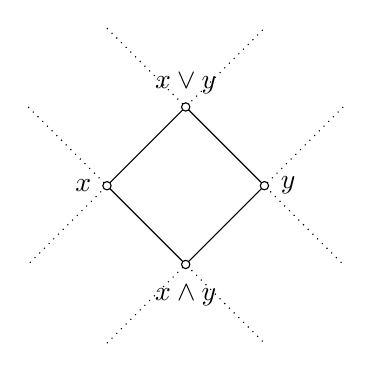
\begin{tikzpicture}
            \draw[dotted] (-1, 1) -- (0, 0) -- (-1, -1);
            \draw (1, 1) -- (0, 0) -- (1, -1);
            \draw (1, 1) -- (2, 0) -- (1, -1);
            \draw[dotted] (0, 2) -- (1, 1) -- (2, 2);
            \draw[dotted] (0, -2) -- (1, -1) -- (2, -2);
            \draw[dotted] (3, 1) -- (2, 0) -- (3, -1);

            \filldraw[color = black, fill = white] (1, 1) circle(1.5pt)
                (1, 1.3) node {$x \jn y$};
            \filldraw[color = black, fill = white] (1, -1) circle(1.5pt)
                (1, -1.4) node {$x \mt y$};
            \filldraw[color = black, fill = white] (0, 0) circle(1.5pt)
                (-0.3, 0) node {$x$};
            \filldraw[color = black, fill = white] (2, 0) circle(1.5pt)
                (2.3, 0) node {$y$};
        \end{tikzpicture}
        }
        \end{figure}
        \pause

        \item $(R, \cdot, 1)$ is a monoid;\pause

        \item for all $x, y, z \in R$,
        \begin{equation}\tag{residuation}\label{res.}
            x \cdot y \leq z \text{ iff } y \leq x \backslash z \text{ iff } x \leq z/y
        \end{equation}
    \end{itemize}
    \pause

For all $x, y, z \in R$
\[
    x(y \vee z) = xy \vee xz \text{ and } (y \vee z) x = yx \vee zx.
\]
\end{frame}

\begin{frame}{Examples of residuated lattices}
%Lattice of (two-sided) ideas of a ring $(\text{Id}(\m R), \cap, +, \cdot_{\text{Id}(\m R)}, \ld, \rd, \m R)$ such that $(\text{Id}(\m R), \cap, +)$ is a complete lattice, $(\text{Id}(\m R), \cdot_{\text{Id}(\m R)}, \m R)$ is a monoid and
%\[
    %A \ld B := \{r \in R: Ar \subseteq B\} \text{ and } B \rd A := \{r \in R: rA \subseteq B\}
%\]

\begin{columns}
    \column{0.5\textwidth}
    $(\bb{Z}, \min, \max, +, -, 0)$ such that $(\bb{Z}, \min, \max)$ is a chain and $(\bb{Z}, +, -, 0)$ is the abelian group on $\bb{Z}$.
    \begin{figure}
        \centering
        \scalebox{0.5}{
        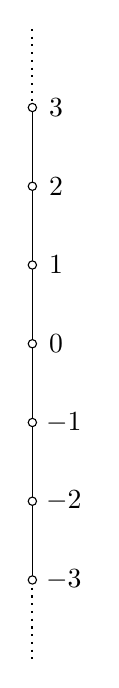
\begin{tikzpicture}
        \draw[thick, dotted] (0, 4) -- (0, 3);
        \draw (0, 3) -- (0, -3);
        \draw[thick, dotted] (0, -3) -- (0, -4);

        \filldraw[color = black, fill = white] (0, 3) circle(1.5pt)
            (0.3, 3) node {$3$};
        \filldraw[color = black, fill = white] (0, 2) circle(1.5pt)
            (0.3, 2) node {$2$};
        \filldraw[color = black, fill = white] (0, 1) circle(1.5pt)
            (0.3, 1) node {$1$};
        \filldraw[color = black, fill = white] (0, 0) circle(1.5pt)
            (0.3, 0) node {$0$};
        \filldraw[color = black, fill = white] (0, -1) circle(1.5pt)
            (0.4, -1) node {$-1$};
        \filldraw[color = black, fill = white] (0, -2) circle(1.5pt)
            (0.4, -2) node {$-2$};
        \filldraw[color = black, fill = white] (0, -3) circle(1.5pt)
            (0.4, -3) node {$-3$};
        \end{tikzpicture}
        }
        \caption{$(\bb{Z}, \min, \max, +, -, 0)$}
    \end{figure}
\pause

\column{0.5\textwidth}
Boolean algebras $(B, \jn, \mt, \neg, 0, 1)$, in which $0$ is the smallest element of the lattice $(B, \jn, \mt)$, $1 = \neg 0$ and (\ref{res.}) becomes
    \[
        x \mt y \leq z \text{ iff } y \leq \neg x \jn z.
    \]
\begin{figure}
    \centering
    \scalebox{0.6}{
    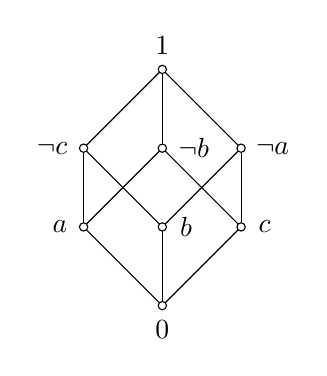
\begin{tikzpicture}
        \draw (1, 2) -- (0, 1) -- (1, 0) -- (2, 1) -- (1, 2);
        \draw (1, 1) -- (0, 0) -- (1, -1) -- (2, 0) -- (1, 1);
        \draw (1, 2) -- (1, 1);
        \draw (0, 1) -- (0, 0);
        \draw (1, 0) -- (1, -1);
        \draw (2, 1) -- (2, 0);

        \filldraw[color = black, fill = white] (1, 2) circle(1.5pt)
            (1, 2.3) node {$1$};
        \filldraw[color = black, fill = white] (1, -1) circle(1.5pt)
            (1, -1.3) node {$0$};
        \filldraw[color = black, fill = white] (0, 0) circle(1.5pt)
            (-0.3, 0) node {$a$};
        \filldraw[color = black, fill = white] (1, 0) circle(1.5pt)
            (1.3, 0) node {$b$};
        \filldraw[color = black, fill = white] (2, 0) circle(1.5pt)
            (2.3, 0) node {$c$};
        \filldraw[color = black, fill = white] (0, 1) circle(1.5pt)
            (-0.4, 1) node {$\neg c$};
        \filldraw[color = black, fill = white] (1, 1) circle(1.5pt)
            (1.4, 1) node {$\neg b$};
        \filldraw[color = black, fill = white] (2, 1) circle(1.5pt)
            (2.4, 1) node {$\neg a$};
    \end{tikzpicture}
    }
    \caption{Boolean algebra $\m 2^3$}
\end{figure}
\end{columns}
\end{frame}

\section{Residuated lattices on \texorpdfstring{$M_X$}{MX}}

\begin{frame}{Residuated lattices on $M_X$}
\begin{columns}
        \column{0.5\textwidth}
            \begin{figure}
            \centering
            \scalebox{0.65}{
                \begin{tikzpicture}
                    \draw[dotted] (0, 2) -- (0, 1);
                    \draw (0, 1) -- (0, -1);
                    \draw[dotted] (0, -1) -- (0, -2);

                    \filldraw[color = black, fill = white] (0, 1) circle (1.5pt);
                    \filldraw[color = black, fill = white] (0, 0) circle (1.5pt)
                        (0.3, 0) node {$1$};
                    \filldraw[color = black, fill = white] (0, -1) circle (1.5pt);
                \end{tikzpicture}
            }
            \caption{A residuated chain}
            \end{figure}

        \pause

        \column{0.5\textwidth}
            \begin{figure}
            \centering
            \scalebox{0.8}{
            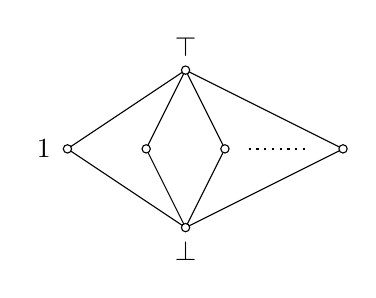
\begin{tikzpicture}
                \draw (1.5, 1) -- (0, 0) -- (1.5, -1);
                \draw (1.5, 1) -- (1, 0) -- (1.5, -1);
                \draw (1.5, 1) -- (2, 0) -- (1.5, -1);
                \draw (1.5, 1) -- (3.5, 0) -- (1.5, -1);
                \draw[thick, dotted] (2.3, 0) -- (3.05, 0);

                \filldraw [color = black, fill = white] (1.5, 1) circle (1.5pt)
                    (1.5, 1.3) node {$\top$};
                \filldraw [color = black, fill = white] (1.5, -1) circle (1.5pt)
                    (1.5, -1.3) node {$\bot$};
                \filldraw [color = black, fill = white] (0, 0) circle (1.5pt)
                    (-0.3, 0) node {$1$};
                \filldraw [color = black, fill = white] (1, 0) circle (1.5pt);
                \filldraw [color = black, fill = white] (2, 0) circle (1.5pt);
                \filldraw [color = black, fill = white] (3.5, 0) circle (1.5pt);
            \end{tikzpicture}
            }
            \caption{A residuated lattice on $M_X$}
            \end{figure}
    \end{columns}
    \pause
    \vspace{20pt}
    
Given a set $X$, we denote by $\mathbf{M}_X$ the lattice over the set $X\cup \{\bot, \top\}$, where $\top$ is the top element, $\bot$ is the bottom element, and $x\vee y=\top$ and $x \wedge y=\bot$, for distinct $x,y \in X$.

\end{frame}

\begin{frame}
    \begin{block}{A well-known result}
        If $X$ is non-empty and closed under multiplication and $\bot$ is absorbing in $M_X$ and $\top$ is absorbing in $X \cup \{\top\}$, then $(X, \cdot, 1)$ is a cancellative monoid.
    \end{block}
    \pause
    \vspace{20pt}

    Proof idea:

    \begin{itemize}
        \item $x (y \jn z) = xy \jn xz$ and $(y \jn z) x = yx \jn zx$;

        \item for $x, y \in X$, $x \neq y$ iff $x \jn y = \top$.
    \end{itemize}
    \pause
    \vspace{20pt}

    Given a residuated lattice on $M_X$, $\top x, x \top \in \{x, \top\}$ for all $x \in X$.

    %A monoid $\mathbf{S}$ with a zero (absorbing element) $0$ is called \emph{$0$-cancellative} if for all $x, y, z \in S$,
    %\begin{align*}
        %xy = xz \neq 0 & \Rightarrow y = z\\
        %yx = zx \neq 0 & \Rightarrow y = z.
    %\end{align*}
    
\end{frame}

\begin{frame}{Properties}
In a residuated lattice $\bf{R}$ on $\mathbf{M}_X$, we define
\begin{align*}
    U_R & = \{x \in R \setminus \{\bot, \top\}: x \top = \top\},\\
    Z_R & = \{x \in R \setminus \{\bot, \top\}: x \top = x\}.
\end{align*}
\pause
\begin{columns}
    \column{0.5\textwidth}
    \begin{figure}
    \centering
    \scalebox{0.7}{
    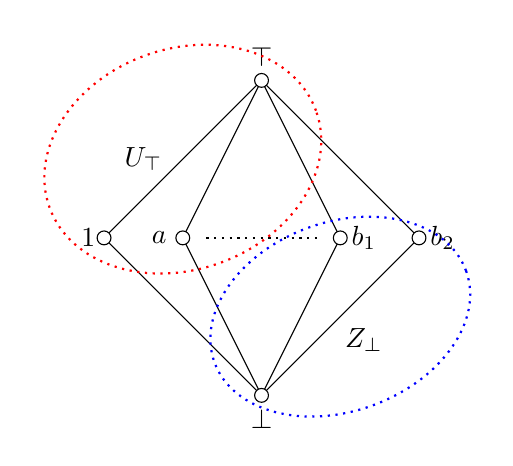
\begin{tikzpicture}
        \draw (2, 2) -- (0, 0) -- (2, -2);
        \draw (2, 2) -- (1, 0) -- (2, -2);
        \draw (2, 2) -- (3, 0) -- (2, -2);
        \draw (2, 2) -- (4, 0) -- (2, -2);
        \draw[thick, dotted] (1.3, 0) -- (2.7, 0);

        \filldraw[color = black, fill = white] (2, 2) circle(2.5pt)
            (2, 2.3) node {$\top$};
        \filldraw[color = black, fill = white] (2, -2) circle(2.5pt)
            (2, -2.3) node {$\bot$};
        \filldraw[color = black, fill = white] (0, 0) circle(2.5pt)
            (-0.2, 0) node {$1$};
        \filldraw[color = black, fill = white] (1, 0) circle(2.5pt)
            (0.7, 0) node {$a$};
        \filldraw[color = black, fill = white] (3, 0) circle(2.5pt)
            (3.3, 0) node {$b_1$};
        \filldraw[color = black, fill = white] (4, 0) circle(2.5pt)
            (4.3, 0) node {$b_2$};

        \draw[red, thick, dotted, rotate around = {20: (1, 1)}] (1, 1) ellipse (1.8 and 1.4);
        \draw[blue, thick, dotted, rotate around = {20: (3, -1)}] (3, -1) ellipse (1.7 and 1.2);

        \draw (0.5, 1) node {$U_{\top}$};
        \draw (3.3, -1.3) node {$Z_{\bot}$};
    \end{tikzpicture}
    }
\end{figure}
\pause

\column{0.5\textwidth}
\begin{itemize}
    \item $\top$ is central in $\mathbf{R}$ and $R = U_R \sqcup Z_R \sqcup \{\bot, \top\}$.
    
    \item $U_{\top} = U_R \cup \{\top\}$.
    
    \item $Z_{\bot} = Z_R \cup \{\bot\}$ and $|Z_{\bot}| \leq 3$.
    
    \item $ab = ba = b$ for all $a \in U_R$ and $b \in Z_R$.
\end{itemize}
\end{columns}

\end{frame}

\begin{frame}{}

\begin{figure}
\centering
\scalebox{0.7}{
\begin{tabular}{c | c}
 & $\bot$\\
\hline
$\bot$ & $\bot$ 
\end{tabular}
\qquad
\begin{tabular}{c | c c}
 & $\bot$ & $b$\\
\hline
$\bot$ & $\bot$ & $\bot$\\
$b$ & $\bot$ & $b$
\end{tabular}
\qquad
\begin{tabular}{c | c c}
 & $\bot$ & $b$\\
\hline
$\bot$ & $\bot$ & $\bot$\\
$b$ & $\bot$ & $\bot$
\end{tabular}
\qquad
\begin{tabular}{c | c c c}
 & $\bot$ & $b_1$ & $b_2$\\
\hline
$\bot$ & $\bot$ & $\bot$ & $\bot$\\
$b_1$ & $\bot$ & $b_1$ & $\bot$\\
$b_2$ & $\bot$ & $\bot$ & $b_2$ 	
\end{tabular}
}
\caption{Multiplication tables of $Z_\bot$}
\label{f:4tables}
\end{figure}

\begin{figure}
    \centering
    \scalebox{0.55}{
    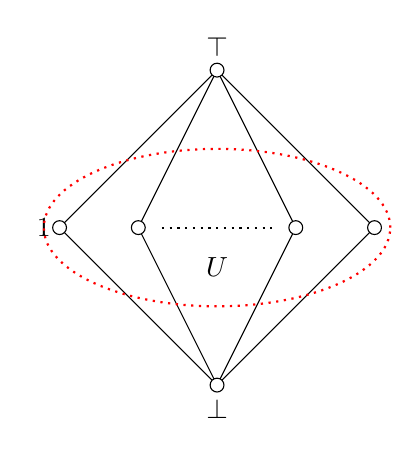
\begin{tikzpicture}
        \draw (2, 2) -- (0, 0) -- (2, -2);
        \draw (2, 2) -- (1, 0) -- (2, -2);
        \draw (2, 2) -- (3, 0) -- (2, -2);
        \draw (2, 2) -- (4, 0) -- (2, -2);
        \draw[thick, dotted] (1.3, 0) -- (2.7, 0);

        \filldraw[color = black, fill = white] (2, 2) circle(2.5pt)
            (2, 2.3) node {$\top$};
        \filldraw[color = black, fill = white] (2, -2) circle(2.5pt)
            (2, -2.3) node {$\bot$};
        \filldraw[color = black, fill = white] (0, 0) circle(2.5pt)
            (-0.2, 0) node {$1$};
        \filldraw[color = black, fill = white] (1, 0) circle(2.5pt);
        \filldraw[color = black, fill = white] (3, 0) circle(2.5pt);
        \filldraw[color = black, fill = white] (4, 0) circle(2.5pt);
        
        \draw[red, thick, dotted] (2, 0) ellipse (2.2 and 1);

        \draw (2, -0.5) node {$U$};
    \end{tikzpicture}
    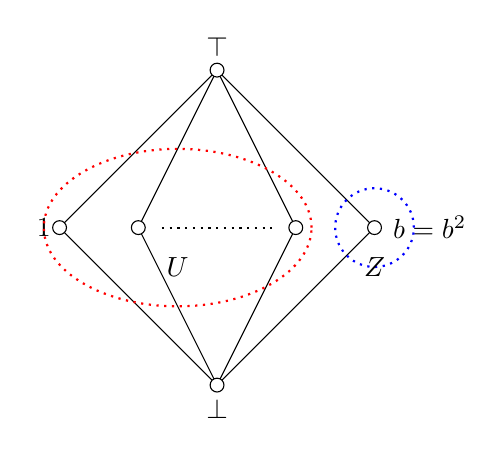
\begin{tikzpicture}
        \draw (2, 2) -- (0, 0) -- (2, -2);
        \draw (2, 2) -- (1, 0) -- (2, -2);
        \draw (2, 2) -- (3, 0) -- (2, -2);
        \draw (2, 2) -- (4, 0) -- (2, -2);
        \draw[thick, dotted] (1.3, 0) -- (2.7, 0);

        \filldraw[color = black, fill = white] (2, 2) circle(2.5pt)
            (2, 2.3) node {$\top$};
        \filldraw[color = black, fill = white] (2, -2) circle(2.5pt)
            (2, -2.3) node {$\bot$};
        \filldraw[color = black, fill = white] (0, 0) circle(2.5pt)
            (-0.2, 0) node {$1$};
        \filldraw[color = black, fill = white] (1, 0) circle(2.5pt);
        \filldraw[color = black, fill = white] (3, 0) circle(2.5pt);
        \filldraw[color = black, fill = white] (4, 0) circle(2.5pt)
            (4.7, 0) node {$b = b^2$};
        
        \draw[red, thick, dotted] (1.5, 0) ellipse (1.7 and 1);
        \draw[blue, thick, dotted] (4, 0) ellipse (0.5 and 0.5);

        \draw (1.5, -0.5) node {$U$};
        \draw (4, -0.5) node {$Z$};
    \end{tikzpicture}
    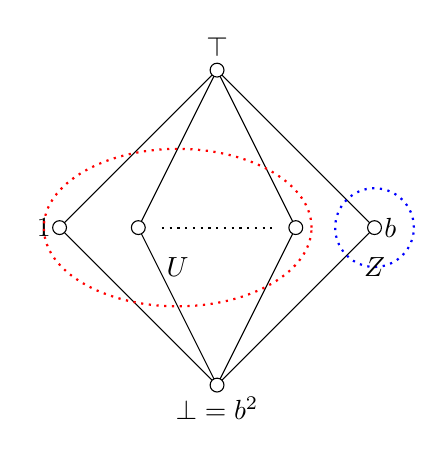
\begin{tikzpicture}
        \draw (2, 2) -- (0, 0) -- (2, -2);
        \draw (2, 2) -- (1, 0) -- (2, -2);
        \draw (2, 2) -- (3, 0) -- (2, -2);
        \draw (2, 2) -- (4, 0) -- (2, -2);
        \draw[thick, dotted] (1.3, 0) -- (2.7, 0);

        \filldraw[color = black, fill = white] (2, 2) circle(2.5pt)
            (2, 2.3) node {$\top$};
        \filldraw[color = black, fill = white] (2, -2) circle(2.5pt)
            (2, -2.3) node {$\bot = b^2$};
        \filldraw[color = black, fill = white] (0, 0) circle(2.5pt)
            (-0.2, 0) node {$1$};
        \filldraw[color = black, fill = white] (1, 0) circle(2.5pt);
        \filldraw[color = black, fill = white] (3, 0) circle(2.5pt);
        \filldraw[color = black, fill = white] (4, 0) circle(2.5pt)
            (4.2, 0) node {$b$};
        
        \draw[red, thick, dotted] (1.5, 0) ellipse (1.7 and 1);
        \draw[blue, thick, dotted] (4, 0) ellipse (0.5 and 0.5);

        \draw (1.5, -0.5) node {$U$};
        \draw (4, -0.5) node {$Z$};
    \end{tikzpicture}
    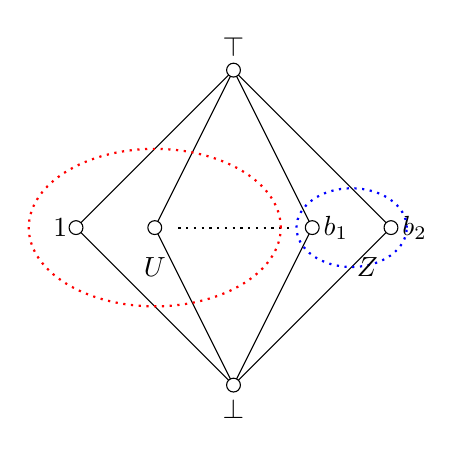
\begin{tikzpicture}
        \draw (2, 2) -- (0, 0) -- (2, -2);
        \draw (2, 2) -- (1, 0) -- (2, -2);
        \draw (2, 2) -- (3, 0) -- (2, -2);
        \draw (2, 2) -- (4, 0) -- (2, -2);
        \draw[thick, dotted] (1.3, 0) -- (2.7, 0);

        \filldraw[color = black, fill = white] (2, 2) circle(2.5pt)
            (2, 2.3) node {$\top$};
        \filldraw[color = black, fill = white] (2, -2) circle(2.5pt)
            (2, -2.3) node {$\bot$};
        \filldraw[color = black, fill = white] (0, 0) circle(2.5pt)
            (-0.2, 0) node {$1$};
        \filldraw[color = black, fill = white] (1, 0) circle(2.5pt);
        \filldraw[color = black, fill = white] (3, 0) circle(2.5pt)
            (3.3, 0) node {$b_1$};
        \filldraw[color = black, fill = white] (4, 0) circle(2.5pt)
            (4.3, 0) node {$b_2$};
        
        \draw[red, thick, dotted] (1, 0) ellipse (1.6 and 1);
        \draw[blue, thick, dotted] (3.5, 0) ellipse (0.7 and 0.5);

        \draw (1, -0.5) node {$U$};
        \draw (3.7, -0.5) node {$Z$};
    \end{tikzpicture}
    }
\caption{Non-linear non-integral residuated lattices over $M_X$}
\end{figure}
\end{frame}

\begin{comment}
\begin{frame}{}
    %\begin{block}{Proposition}
        %In any residuated lattice $\mathbf{R}$ with top $\top$, the set $R_\top = Z_R \cup \{\top, \bot\}$ is a subalgebra of $\mathbf{R}$ with respect to all operations other than $1$, and $\top$ is a multiplicative identity for $R_\top$.
        %Hence, $\bf{R}_\top$ is an integral residuated lattice.
    %\end{block}
    
    \begin{figure}
        \centering
        \begin{tikzpicture}
            \draw (0, 1) -- (0, 0);
            %\draw (0, -0.8) node {$2$-element generalized Boolean algebra};

            \filldraw[color = black, fill = white] (0, 1) circle (1.5pt)
                (0, 1.3) node {$\top = 1$};
            \filldraw[color = black, fill = white] (0, 0) circle (1.5pt)
                (0, -0.3) node {$\bot$};
        \end{tikzpicture}
        \quad
        \begin{tikzpicture}
            \draw (0, 1) -- (0, -1);
            %\draw (0, -1.8) node {$3$-element generalized Brouwerian algebra};

            \filldraw[color = black, fill = white] (0, 1) circle (1.5pt)
                (0, 1.3) node {$\top = 1$};
            \filldraw[color = black, fill = white] (0, -1) circle (1.5pt)
                (0, -1.3) node {$\bot$};
            \filldraw[color = black, fill = white] (0, 0) circle (1.5pt)
                (0.7, 0) node {$b = b^2$};
        \end{tikzpicture}
        \quad
        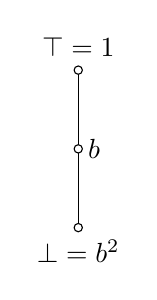
\begin{tikzpicture}
            \draw (0, 1) -- (0, -1);
            %\draw (0, -1.8) node {$3$-element generalized MV-algebra};

            \filldraw[color = black, fill = white] (0, 1) circle (1.5pt)
                (0, 1.3) node {$\top = 1$};
            \filldraw[color = black, fill = white] (0, -1) circle (1.5pt)
                (0, -1.3) node {$\bot = b^2$};
            \filldraw[color = black, fill = white] (0, 0) circle (1.5pt)
                (0.2, 0) node {$b$};
        \end{tikzpicture}
        \quad
        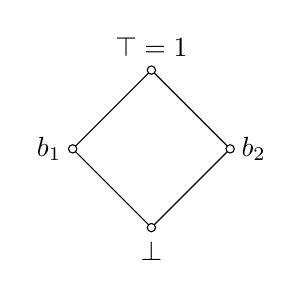
\begin{tikzpicture}
            \draw (1, 1) -- (0, 0) -- (1, -1);
            \draw (1, 1) -- (2, 0) -- (1, -1);
            %\draw (1, -1.8) node {$4$-element generalized Boolean algebra};

            \filldraw[color = black, fill = white] (1, 1) circle (1.5pt)
                (1, 1.3) node {$\top = 1$};
            \filldraw[color = black, fill = white] (1, -1) circle (1.5pt)
                (1, -1.3) node {$\bot$};
            \filldraw[color = black, fill = white] (0, 0) circle (1.5pt)
                (-0.3, 0) node {$b_1$};
            \filldraw[color = black, fill = white] (2, 0) circle (1.5pt)
                (2.3, 0) node {$b_2$};
        \end{tikzpicture}
        \caption{Integral residuated lattices:\\
        (a) $2$-element generalized Boolean algebra;\\
        (b) $3$-element generalized Brouwerian algebra;\\
        (c) $3$-element generalized MV-algebra;\\
        (d) $4$-element generalized Boolean algebra}
    \end{figure}
\end{frame}
\end{comment}


%\begin{frame}{Construction and Characterization}

%Let $\mathbf{A}$ be $\top$-cancellative monoid with zero $\top$ and $\mathbf{B}$ be a semigroup with zero $\bot$, whose multiplication table is one of those in Figure~\ref{f:4tables}.\pause
%We define the lattice structure $\mathbf{M}_X$ on the set $R = A \cup B$, where $X = R \setminus \{\bot, \top\}$, $\bot$ is the bottom and $\top$ is the top. \pause
%Also, we define a multiplication on $R$ that extends the multiplications on $\mathbf{A}$ and $\mathbf{B}$ by: $xy = yx = y$, for all $x \in A$ and $y \in B$.
%We denote by $\mathbf{R}_{\mathbf{A}, \mathbf{B}}$ the resulting algebra.
%\end{frame}

\begin{frame}{Construction and Characterization}
\begin{columns}
    \column{0.5\textwidth}
    \begin{figure}
    \centering
    \scalebox{0.8}{
    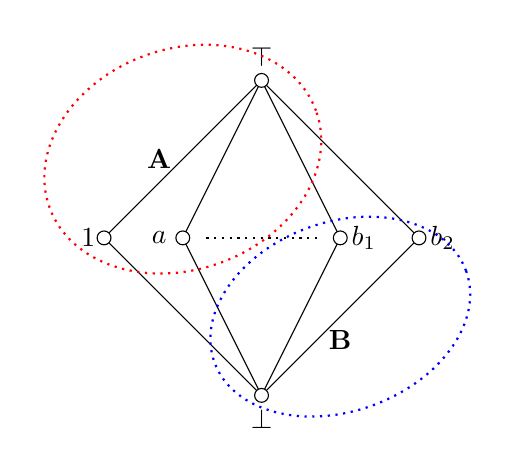
\begin{tikzpicture}
        \draw (2, 2) -- (0, 0) -- (2, -2);
        \draw (2, 2) -- (1, 0) -- (2, -2);
        \draw (2, 2) -- (3, 0) -- (2, -2);
        \draw (2, 2) -- (4, 0) -- (2, -2);
        \draw[thick, dotted] (1.3, 0) -- (2.7, 0);

        \filldraw[color = black, fill = white] (2, 2) circle(2.5pt)
            (2, 2.3) node {$\top$};
        \filldraw[color = black, fill = white] (2, -2) circle(2.5pt)
            (2, -2.3) node {$\bot$};
        \filldraw[color = black, fill = white] (0, 0) circle(2.5pt)
            (-0.2, 0) node {$1$};
        \filldraw[color = black, fill = white] (1, 0) circle(2.5pt)
            (0.7, 0) node {$a$};
        \filldraw[color = black, fill = white] (3, 0) circle(2.5pt)
            (3.3, 0) node {$b_1$};
        \filldraw[color = black, fill = white] (4, 0) circle(2.5pt)
            (4.3, 0) node {$b_2$};

        \draw[red, thick, dotted, rotate around = {20: (1, 1)}] (1, 1) ellipse (1.8 and 1.4);
        \draw[blue, thick, dotted, rotate around = {20: (3, -1)}] (3, -1) ellipse (1.7 and 1.2);

        \draw (0.7, 1) node {$\m A$};
        \draw (3, -1.3) node {$\m B$};
    \end{tikzpicture}
    }
\caption{$R_{\m A, \m B}$}
\end{figure}
\pause

\column{0.5\textwidth}
    The residuated lattices based on $\mathbf{M}_X$ are precisely the ones of the form $\mathbf{R}_{\mathbf{A}, \mathbf{B}}$ and the integral ones.
\end{columns}

\end{frame}

\begin{comment}
\begin{frame}
\begin{block}{Theorem}
    $\mathbf{R}_{\mathbf{A}, \mathbf{B}}$ is the reduct of a residuated lattice based on $\mathbf{M}_X$, where $X = A \cup B \setminus \{\bot, \top\}$.
\end{block}
\pause

\begin{block}{Corollary}
    The residuated lattices based on $\mathbf{M}_X$ are precisely the ones of the form $\mathbf{R}_{\mathbf{A}, \mathbf{B}}$, where $\mathbf{A}$ is a $\top$-cancellative monoid with zero $\top$ and $\mathbf{B}$ is a semigroup with zero $\bot$, whose multiplication table is one of those in Figure~\ref{f:4tables}; and integral ones: $2$-element Boolean algebra, $3$-element Heyting algebra, $3$-element MV-algebra and $4$-element Boolean algebra.
\end{block}
\end{frame}
\end{comment}

\begin{frame}{Subvarieties of $\mathsf{M}$}
    A variety $\mathcal{V}$ is a class of algebras that is closed under class operation $H$ (homomorphic images), $S$ (subalgebras) and $P$ (direct products).\pause
    \medskip

    Examples of varieties:
    \begin{itemize}
        \item The class of all groups is a variety.

        \item The class of all abelian groups is a variety.

        \item The class of all lattices is a variety.

        \item The class of all chains is \emph{not} a variety.
    \end{itemize}

    \begin{block}{Theorem}
        The variety $\mathsf{M}$ generated by the class of residuated lattices on $M_X$ has uncountably-many subvarieties.
    \end{block}
\end{frame}

\begin{frame}{Proof idea (continue)}
    %Subclasses of $HSP_U(\{\m {M_G}: \m G \in \mathsf{AG}\})$ bijectively corresponds to subclasses $HS(\{\m {M_G}: \m G \in P_U(\mathsf{AG})\})$, which also bijectively corresponds to subclasses of $H(\{\m {M_G}: \m G \in SP_U(\mathsf{AG})\})$.\pause
    %\medskip

    %Since each $\m {M_G}$ is simple, $H(\{\m {M_G}: \m G \in SP_U(\mathsf{AG})\})$ is the same as $I(\{\m {M_G}: \m G \in SP_U(\mathsf{AG})\})$, and subclasses of $H(\{\m {M_G}: \m G \in SP_U(\mathsf{AG})\})$ corresponds to subclasses of $\{\m {M_G}: \m G \in ISP_U(\mathsf{AG})\}$.\pause
    %\medskip

    Proof idea: We focus on the subvarieties of the variety $\mathsf{CM_G}$ generated by $\m {M_G}$, where $\m G$ is an abelian group.\pause
    \medskip
    
    Every class of \emph{subdirectly irreducible} algebras of $\mathsf{CM_G}$ is a subclass of $HSP_U(\{\m {M_G}: \m G \in \mathsf{AG}\})$.
    \begin{align*}
        HSP_U(\{\m {M_G}: \m G \in \mathsf{AG}\}) & = HS(\{\m {M_G}: \m G \in P_U \text{-subclasses of } \mathsf{AG}\})\\
        & = H(\{\m {M_G}: \m G \in {SP_U} \text{-subclasses of } \mathsf{AG}\})\\
        & = I(\{\m {M_G}: \m G \in {SP_U} \text{-subclasses of } \mathsf{AG}\})\\
        & \leftrightarrow \{\m {M_G}: \m G \in {ISP_U} \text{-subclasses of } \mathsf{AG}\}
    \end{align*}
    \pause
    So the lattice of subvarieties of $\mathsf{CM_G}$ is isomorphic to the lattice of $(ISP_U)$-subclasses of $\mathsf{AG}$.
\end{frame}

\begin{frame}{Proof idea (continue)}
    \begin{block}{}
        Every algebra can be embedded into an ultraproduct of its finitely generated subalgebras.
    \end{block}
    \pause
    \medskip
    
    \begin{block}{Fundamental theorem of finitely generated abelian groups}
        Every finitely generated abelian group is isomorphic to exactly one group of the form
        \[
            \mathbb{Z}^m \times (\mathbb{Z}_{p_1^{n_{1, 1}}} \times \cdots \times \mathbb{Z}_{p_1^{n_{1,m_1}}}) \times \cdots \times (\mathbb{Z}_{p_k^{n_{k, 1}}} \times \cdots \times \mathbb{Z}_{p_k^{n_{k,m_k}}})  
        \]
        for some $m, k, m_1, \dots, m_k,n_{i,j} \in \mathbb{N}$, where $n_{i,j} \geq n_{i,j+1}$ for all suitable $i, j$, and $p_1 < p_2 < \dots < p_k < \ldots $ is the listing of all primes.
    \end{block}    
\end{frame}

\begin{frame}{Proof idea (continue)}
    \begin{align*}
        \mathbb{Z}^2 \times (\mathbb{Z}_{2^4} \times \bb{Z}_{2^2} \times \bb{Z}_2) \times (\bb{Z}_{3^3} \times \bb{Z}_{3^2}) & \leftrightarrow (2; 4, 2, 1; 3, 2; 0; \dots)\\
        \mathbb{Z}^5 \times \mathbb{Z}_{3^2} \times (\bb{Z}_{5^3} \times \bb{Z}_{5^2}) \times (\bb{Z}_{7^5} \times \bb{Z}_{7^3}) & \leftrightarrow (5; 0; 2; 3, 2; 5, 3; 0; \dots)\\
        (\mathbb{Z}_{2^6} \times \mathbb{Z}_{2^4} \times \mathbb{Z}_2) \times (\bb{Z}_{5^5} \times \bb{Z}_{5^2}) \times \bb{Z}_7 & \leftrightarrow (0; 6, 4, 1; 0; 5, 2; 1; 0; \dots)
    \end{align*}
    \pause
    $\m G \times \mathbb{Z}^r \in \mathcal{K}$ iff $\m G \times \mathbb{Z}^s \in \mathcal{K}$ for $r, s \in \bb{Z}^+$, where $\m G$ is a finite abelian group and $\mathcal{K}$ an $\mathsf{ISP_U}$-class of abelian groups.\pause
    \medskip

    \begin{block}{Theorem}
        The lattice of subvarieties of $\mathsf{CM_G}$ is isomorphic to $\mathcal{O}_{\bb{Z}}(\m P)$.
    \end{block}
\end{frame}

\section{Axiomatization}

\begin{frame}{Axioms for the class of residuated lattices on $M_X$}

A class $\mathcal{V}$ is a variety iff it is an equational class, i.e., there exists a set of equations such that only algebras in $\mathcal{V}$ satisfy them.

\begin{figure}
\centering
\scalebox{0.7}{
    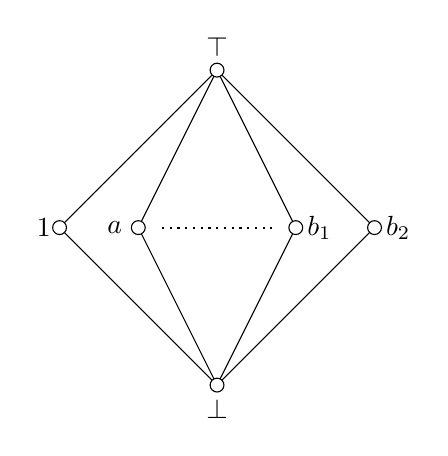
\begin{tikzpicture}
        \draw (2, 2) -- (0, 0) -- (2, -2);
        \draw (2, 2) -- (1, 0) -- (2, -2);
        \draw (2, 2) -- (3, 0) -- (2, -2);
        \draw (2, 2) -- (4, 0) -- (2, -2);
        \draw[thick, dotted] (1.3, 0) -- (2.7, 0);

        \filldraw[color = black, fill = white] (2, 2) circle(2.5pt)
            (2, 2.3) node {$\top$};
        \filldraw[color = black, fill = white] (2, -2) circle(2.5pt)
            (2, -2.3) node {$\bot$};
        \filldraw[color = black, fill = white] (0, 0) circle(2.5pt)
            (-0.2, 0) node {$1$};
        \filldraw[color = black, fill = white] (1, 0) circle(2.5pt)
            (0.7, 0) node {$a$};
        \filldraw[color = black, fill = white] (3, 0) circle(2.5pt)
            (3.3, 0) node {$b_1$};
        \filldraw[color = black, fill = white] (4, 0) circle(2.5pt)
            (4.3, 0) node {$b_2$};
    \end{tikzpicture}
}
    \qquad \qquad
    \begin{tikzpicture}
        \draw (0, 1) -- (0, -1);

        \filldraw[color = black, fill = white] (0, 1) circle(1.5pt)
            (0, 1.3) node {$\top$};
        \filldraw[color = black, fill = white] (0, -1) circle(1.5pt)
            (0, -1.3) node {$\bot = b^2$};
        \filldraw[color = black, fill = white] (0, 0) circle(1.5pt)
            (0.3, 0) node {$b$};
    \end{tikzpicture}
\caption{Non-linear and linear residuated lattices on $M_X$}
\end{figure}
\end{frame}

\begin{frame}{Axiom (URL)}
    
    A (bounded) residuated lattice is called \emph{unilinear} if it satisfies 
    \begin{equation}\tag{URL}\label{axiom_URL}
        \begin{split}
            \forall x, y \, (x \leq y & \text{ or } y \leq x \text{ or } (x \mt y = \bot \text{ and } x \jn y = \top)).
        \end{split}        
    \end{equation}
    \pause
    To include unbounded chains, we can have
    \begin{align*}
        \forall x, y, z, w \, (x \leq y \text{ or } y \leq x \text{ or } (x \mt y \leq z \text{ and } w \leq x \jn y))
    \end{align*}
    \pause

    \begin{figure}
    \centering
    \scalebox{0.4}{
    \begin{tikzpicture}
        \draw (3, 4) -- (0, 3);
        \draw[dotted] (0, 3) -- (0, -3);
        \draw (0, -3) -- (3, -4);
        \draw (3, 4) -- (1.5, 3);
        \draw[dotted] (1.5, 3) -- (1.5, -3);
        \draw (1.5, -3) -- (3, -4);
        \draw[dotted] (2, 0) -- (5.5, 0);
        \draw (3, 4) -- (6, 3);
        \draw[dotted] (6, 3) -- (6, -3);
        \draw (6, -3) -- (3, -4);

        \filldraw [color = black, fill = white] (3, 4) circle (2.5pt)
            (3, 4.4) node {$\top$};
        \filldraw [color = black, fill = white] (3, -4) circle (2.5pt)
            (3, -4.4) node [black] {$\bot$};
        \filldraw [color = black, fill = white] (0, 2) circle (2.5pt)
            (-0.3, 2.3) node [black] {};
        \filldraw [color = black, fill = white] (0, 1) circle (2.5pt)
            (-0.3, 1.3) node [black] {};
        \filldraw [color = black, fill = white] (0, 0) circle (2.5pt)
            (-0.3, 0.3) node [black] {};
        \filldraw [color = black, fill = white] (0, -1) circle (2.5pt)
            (-0.4, -0.7) node [black] {};
        \filldraw [color = black, fill = white] (0, -2) circle (2.5pt)
            (-0.4, -1.7) node [black] {};

        \filldraw [color = black, fill = white] (1.5, 2) circle (2.5pt);
        \filldraw [color = black, fill = white] (1.5, 1) circle (2.5pt);
        \filldraw [color = black, fill = white] (1.5, 0) circle (2.5pt)
            (1.2, 0.3) node {};
        \filldraw [color = black, fill = white] (1.5, -1) circle (2.5pt);
        \filldraw [color = black, fill = white] (1.5, -2) circle (2.5pt);

        \filldraw [color = black, fill = white] (6, 2) circle (2.5pt);
        \filldraw [color = black, fill = white] (6, 1) circle (2.5pt);
        \filldraw [color = black, fill = white] (6, 0) circle (2.5pt)
            (6.3, 0.3) node [black] {};
        \filldraw [color = black, fill = white] (6, -1) circle (2.5pt);
        \filldraw [color = black, fill = white] (6, -2) circle (2.5pt);
    \end{tikzpicture}
    }
    \qquad \qquad
    \scalebox{0.6}{
    
\begin{tikzpicture}
        \draw[thick, dotted] (0, 3) -- (0, 2);
        \draw (0, 2) -- (0, -2);
        \draw[thick, dotted] (0, -2) -- (0, -3);

        \filldraw[color = black, fill = white] (0, 2) circle(2.5pt);
        \filldraw[color = black, fill = white] (0, 1) circle(2.5pt);
        \filldraw[color = black, fill = white] (0, 0) circle(2.5pt);
        \filldraw[color = black, fill = white] (0, -1) circle(2.5pt);
        \filldraw[color = black, fill = white] (0, -2) circle(2.5pt);
    \end{tikzpicture}
    }
    \end{figure}
        
\end{frame}

\begin{frame}{Axiom ($h_n$)}

    A (bounded) residuated lattice has height at most $n$ iff it satisfies
    \begin{equation}\tag{$h_n$}\label{axiom_of_finite_height}
            \forall x_1, \dots, x_{n+1} \, (\bigor \limits_{1 \leq m \leq n}
            x_1 \vee \dots \vee x_{m} = x_1 \vee \dots \vee x_{m+1}).
    \end{equation}

    In particular, $(h_3)$ is the universal closure of 
    $$x_1 = x_1 \vee x_2 \text{ or } x_1 \vee x_2 = x_1 \vee x_2 \vee x_3 \text{ or } x_1 \vee x_2 \vee x_3 = x_1 \vee x_2 \vee x_3 \vee x_4.$$

    \pause

    The class of residuated lattices over $M_X$ is axiomatized by (\ref{axiom_URL}) and ($h_3$) and we denote this class by $\mathsf{URL_3}$.
    We also denote the class of residuated lattices satisfying (\ref{axiom_URL}) by $\mathsf{URL}$.
\end{frame}

\begin{comment}
\begin{frame}{Varieties $\mathsf{SRL}$ and $\mathsf{M}$}
    A variety $\mathcal{V}$ is a class of algebras which is closed under the class operations $H$ (homomorphisms), $S$ (subalgebras) and $P$ (direct product).\pause
    A variety is an equational class, i.e., each algebra in the variety satisfies a fixed set of equations.\pause
    \medskip
    
    Let $\m R$ be a residuated lattice and $a, x \in R$.
    The \emph{left conjugate} of $a$ by $x$ is the term $x \ld ax \mt 1$ and the \emph{right conjugate} is $xa \rd x \mt 1$; \emph{iterated conjugates} are obtained by repeated applications of left and right conjugates by various conjugating elements from the set $\text{Var}$ of variables.
    Here we use $\Gamma(\text{Var})$ to denote the set of all iterated conjugates by elements from set $\text{Var}$.
\end{frame}
\end{comment}

\begin{comment}
\begin{frame}{Equational basis for $\mathsf{SRL}$ and $\mathsf{M}$}
    \begin{align*}
        & \forall x, y \, (x \leq y \text{ or } y \leq x)\\\pause
        & \forall x, y \, (1 \leq x \ld y \text{ or } 1 \leq y \ld x)\\\pause
        & \forall x, y \, (1 = (x \ld y) \mt 1 \text{ or } 1 = (y \ld x) \mt 1)\\\pause
        & \forall x, y \, (1 = \gamma_1((x \ld y) \mt 1) \jn \gamma_2((y \ld x) \mt 1))
    \end{align*}
    
    $\gamma_1 = \lambda_{x_1} \circ \rho_{x_2} \circ \rho_{x_3} \circ \lambda_{x_4} \circ \cdots$ and $\lambda_{x_1}(a) = (x_1 \ld a x_1) \mt 1$, $\rho_{x_2}(a) = (x_2 a \rd x_2) \mt 1$.
\end{frame}
\end{comment}

\begin{frame}{Equational basis for $\mathsf{SRL}$ and $\mathsf{M}$}
    By \cite{galatos2004equational}, the variety of semiunilinear residuated lattices, $\mathsf{SRL}$, generated by the class $\mathsf{URL}$, is axiomatized by the equations
    \begin{align*}
        1 & = \gamma_1(u_1 \backslash u_2) \vee \gamma_2(u_2 \backslash u_1) \vee \gamma_3 ((u_1 \wedge u_2) \backslash x)\\
        1 & = \gamma_4(u_1 \backslash u_2) \vee \gamma_5(u_2 \backslash u_1) \vee \gamma_6 (y \backslash (u_1 \vee u_2)),
    \end{align*}
    where $ \gamma_1, \gamma_2, \gamma_3, \gamma_4, \gamma_5, \gamma_6 \in \Gamma(\text{Var})$.\pause
    \medskip

    The variety $\mathsf{M}$ generated by $\mathsf{URL_3}$, is axiomatized by the semiunilinear equations together with the equations 
    \begin{align*}
        1 = \gamma_1((x_1 \vee x_2)\backslash x_1) \vee & \gamma_2((x_1 \vee x_2 \vee x_3)\backslash (x_1 \vee x_2))\\
        \vee & \gamma_3((x_1 \vee x_2 \vee x_3 \vee x_4) \backslash (x_1 \vee x_2 \vee x_3)),
    \end{align*}
    where $\gamma_1, \gamma_2, \gamma_3 \in \Gamma(\text{Var})$.
\end{frame}

\begin{comment}
\begin{frame}{Finitely subdirectly irreducible algebras in $\mathsf{SRL}$ and $\mathsf{M}$}
    Given a variety $\mathcal{V}$, an algebra $\m A \in \mathcal{V}$ is called (finitely) subdirectly-irreducible if whenever $\m A$ is isomorphic to a subdirect product of a (non-empty finite) set of algebras in $\mathcal{V}$, it is isomorphic to one of these algebras.
    We use $\mathcal{V}_{FSI}$ and $\mathcal{V}_{SI}$ to denote the classes of finitely subdireclty irreducible and subdireclty irreducible members in $\mathcal{V}$ respectively.\pause
    \medskip

    Every algebra in a variety $\mathcal{V}$ is a subalgebra of the direct product of the subdireclty-irreducible members, so $\mathcal{V} = HSP(\mathcal{V}_{SI}) = HSP(\mathcal{V}_{FSI})$.
\end{frame}
\end{comment}

\begin{frame}{Finitely subdirectly irreducible algebras in $\mathsf{SRL}$ and $\mathsf{M}$}

By the corresponding theorem in \cite{galatos2007residuated}, we know all unilinear residuated lattices are finitely subdirectly-irreducible members in $\mathsf{SRL}$, i.e., $\mathsf{URL} \subseteq \mathsf{SRL}_{FSI}$.\pause
\medskip

By \cite{galatos2004equational}, the class of finitely subdirectly-irreducible members of $\mathsf{SRL}$ is precisely the class of unilinear residuated lattice.
\medskip

\begin{block}{Theorem}\label{t: FSI}
$\mathsf{SRL}_{FSI} = \mathsf{URL}$ and $\mathsf{M}_{SI} = \mathsf{M}_{FSI} = \mathsf{URL_3}$.
\end{block}
\end{frame}

\section{Unilinear residuated lattices}

\begin{comment}
\begin{frame}{Unilinear residuated lattices}

A residuated lattice is \emph{unilinear} if it satisfies (\ref{axiom_URL}).\pause
    
    \begin{figure}
    \centering
    \scalebox{0.7}{
    
\begin{tikzpicture}
        \draw[thick, dotted] (0, 3) -- (0, 2);
        \draw (0, 2) -- (0, -2);
        \draw[thick, dotted] (0, -2) -- (0, -3);

        \filldraw[color = black, fill = white] (0, 2) circle(2.5pt);
        \filldraw[color = black, fill = white] (0, 1) circle(2.5pt);
        \filldraw[color = black, fill = white] (0, 0) circle(2.5pt);
        \filldraw[color = black, fill = white] (0, -1) circle(2.5pt);
        \filldraw[color = black, fill = white] (0, -2) circle(2.5pt);
    \end{tikzpicture}
    }
    \qquad \qquad \qquad
    \scalebox{0.55}{
    \begin{tikzpicture}
        \draw (3, 4) -- (0, 3);
        \draw[dotted] (0, 3) -- (0, -3);
        \draw (0, -3) -- (3, -4);
        \draw (3, 4) -- (1.5, 3);
        \draw[dotted] (1.5, 3) -- (1.5, -3);
        \draw (1.5, -3) -- (3, -4);
        \draw[dotted] (2, 0) -- (5.5, 0);
        \draw (3, 4) -- (6, 3);
        \draw[dotted] (6, 3) -- (6, -3);
        \draw (6, -3) -- (3, -4);

        \filldraw [color = black, fill = white] (3, 4) circle (2.5pt)
            (3, 4.4) node {$\top$};
        \filldraw [color = black, fill = white] (3, -4) circle (2.5pt)
            (3, -4.4) node [black] {$\bot$};
        \filldraw [color = black, fill = white] (0, 2) circle (2.5pt)
            (-0.3, 2.3) node [black] {};
        \filldraw [color = black, fill = white] (0, 1) circle (2.5pt)
            (-0.3, 1.3) node [black] {};
        \filldraw [color = black, fill = white] (0, 0) circle (2.5pt)
            (-0.3, 0.3) node [black] {};
        \filldraw [color = black, fill = white] (0, -1) circle (2.5pt)
            (-0.4, -0.7) node [black] {};
        \filldraw [color = black, fill = white] (0, -2) circle (2.5pt)
            (-0.4, -1.7) node [black] {};

        \filldraw [color = black, fill = white] (1.5, 2) circle (2.5pt);
        \filldraw [color = black, fill = white] (1.5, 1) circle (2.5pt);
        \filldraw [color = black, fill = white] (1.5, 0) circle (2.5pt)
            (1.2, 0.3) node {};
        \filldraw [color = black, fill = white] (1.5, -1) circle (2.5pt);
        \filldraw [color = black, fill = white] (1.5, -2) circle (2.5pt);

        \filldraw [color = black, fill = white] (6, 2) circle (2.5pt);
        \filldraw [color = black, fill = white] (6, 1) circle (2.5pt);
        \filldraw [color = black, fill = white] (6, 0) circle (2.5pt)
            (6.3, 0.3) node [black] {};
        \filldraw [color = black, fill = white] (6, -1) circle (2.5pt);
        \filldraw [color = black, fill = white] (6, -2) circle (2.5pt);
    \end{tikzpicture}
    }
    \caption{Linear and non-linear URLs}
    \end{figure}
\end{frame}
\end{comment}

\begin{frame}{Unilinear residuated lattices}

    Let $\m R$ be a non-linear unilinear residuated lattice, define
    \begin{align*}
        U_R & = \{x \in R \setminus \{\bot, \top\}: x \top = \top\},\\
        Z_R & = \{x \in R \setminus \{\bot, \top\}: x \top = x\},\\
        W_R & = \{x \in R \setminus \{\bot, \top\}: x < x \top < \top\}.
    \end{align*}
    \pause

    \begin{block}{Theorem}\label{T-central}
        Every non-linear unilinear residuated lattice is $\top$-central, i.e., for each element $x$, $\top x = x \top$.
    \end{block}
    \medskip

    \begin{center}
        $R = U_R \sqcup Z_R \sqcup W_R \sqcup \{\bot, \top\}$ 
    \end{center}
    
\end{frame}

\begin{comment}
\begin{frame}{}
    \begin{itemize}
        \item Where are the products among $U_R$, $Z_R$ and $W_R$?\pause

        \item What are the positions for $U_R$, $Z_R$ and $W_R$?
    \end{itemize}
    
    %$R_{\top} = Z_R \cup \{\bot, \top\}$ is a $1$-free subalgebra of $\m R$;\pause
    %$Z_R$ is either linear or a $2$-element antichain;\pause
    %in most cases, $U_R \cup \{\bot, \top\}$ is a subalgebra;\pause
    %elements in $W_R$ are incomparable with those in $U_R$;\pause
    %when $W_R \neq \emptyset$, $W_R$ is a chain of the downset of the least such elements in $Z_R$ that is incomparable with $1$.
\end{frame}

\begin{frame}{Class $\mathsf{Tunital}$}
    This is the class of all the URLs satisfying
    \[
        \forall x \, (x = \bot \text{ or } \top x = \top).
    \]
    \pause
    
    If $\m R$ is a non-linear member in $\mathsf{Tunital}$, then $U_R = R \setminus \{\bot, \top\}$.
    \begin{center}
        \scalebox{0.4}{
        \begin{tikzpicture}
        \draw (3, 4) -- (0, 3);
        \draw[dotted] (0, 3) -- (0, -3);
        \draw (0, -3) -- (3, -4);
        \draw (3, 4) -- (1.5, 3);
        \draw[dotted] (1.5, 3) -- (1.5, -3);
        \draw (1.5, -3) -- (3, -4);
        \draw[dotted] (2, 0) -- (5.5, 0);
        \draw (3, 4) -- (6, 3);
        \draw[dotted] (6, 3) -- (6, -3);
        \draw (6, -3) -- (3, -4);

        \draw[thick, dotted] (3, 0) ellipse (4 and 3.7);

        \draw (3, -1) node {$U_R$};

        \filldraw [color = black, fill = white] (3, 4) circle (2.5pt)
            (3, 4.4) node {$\top$};
        \filldraw [color = black, fill = white] (3, -4) circle (2.5pt)
            (3, -4.4) node [black] {$\bot$};
        \filldraw [color = black, fill = white] (0, 2) circle (2.5pt)
            (-0.3, 2.3) node [black] {};
        \filldraw [color = black, fill = white] (0, 1) circle (2.5pt)
            (-0.3, 1.3) node [black] {};
        \filldraw [color = black, fill = white] (0, 0) circle (2.5pt)
            (-0.3, 0.3) node [black] {};
        \filldraw [color = black, fill = white] (0, -1) circle (2.5pt)
            (-0.4, -0.7) node [black] {};
        \filldraw [color = black, fill = white] (0, -2) circle (2.5pt)
            (-0.4, -1.7) node [black] {};

        \filldraw [color = black, fill = white] (1.5, 2) circle (2.5pt);
        \filldraw [color = black, fill = white] (1.5, 1) circle (2.5pt);
        \filldraw [color = black, fill = white] (1.5, 0) circle (2.5pt)
            (1.2, 0.3) node {};
        \filldraw [color = black, fill = white] (1.5, -1) circle (2.5pt);
        \filldraw [color = black, fill = white] (1.5, -2) circle (2.5pt);

        \filldraw [color = black, fill = white] (6, 2) circle (2.5pt);
        \filldraw [color = black, fill = white] (6, 1) circle (2.5pt);
        \filldraw [color = black, fill = white] (6, 0) circle (2.5pt)
            (6.3, 0.3) node [black] {};
        \filldraw [color = black, fill = white] (6, -1) circle (2.5pt);
        \filldraw [color = black, fill = white] (6, -2) circle (2.5pt);
        \end{tikzpicture}
        }
    \end{center}
\end{frame}

\begin{frame}{Class $\mathsf{B}$}
    In this class, the non-linear members are axiomatized by
    \begin{align}
        & \forall x \, (\overline{\top} x = \overline{\top} \text{ or } \overline{\top} x = x) \tag{$W\emptyset$} \label{Wempty}\\
        & \overline{\top} \backslash 1 = \overline{\bot} \tag{$b \parallel 1$} \label{b_incomparable_with_1}\\
        & \forall x \, (\overline{\top} x = \overline{\top} \text{ or } x \backslash \overline{\bot} \vee x = \overline{\top}) \tag{ZBoolean} \label{4Boolean}
    \end{align}

    \begin{center}
        \scalebox{0.4}{
        \begin{tikzpicture}
        \draw (3, 4) -- (0, 3);
        \draw[dotted] (0, 3) -- (0, -3);
        \draw (0, -3) -- (3, -4);
        \draw (3, 4) -- (1.5, 3);
        \draw[dotted] (1.5, 3) -- (1.5, -3);
        \draw (1.5, -3) -- (3, -4);
        \draw[dotted] (2, 0) -- (4, 0);
        \draw (3, 4) -- (4.5, 0) -- (3, -4);
        \draw (3, 4) -- (6, 0) -- (3, -4);

        \filldraw [color = black, fill = white] (3, 4) circle (2.5pt)
            (3, 4.3) node {$\top$};
        \filldraw [color = black, fill = white] (3, -4) circle (2.5pt)
            (3, -4.3) node [black] {$\bot$};
        \filldraw [color = black, fill = white] (0, 2) circle (2.5pt)
            (-0.3, 2) node [black] {$a_n$};
        \filldraw [color = black, fill = white] (0, 1) circle (2.5pt)
            (-0.3, 1) node [black] {$a_1$};
        \filldraw [color = black, fill = white] (0, 0) circle (2.5pt)
            (-0.2, 0) node [black] {$1$};
        \filldraw [color = black, fill = white] (0, -1) circle (2.5pt)
            (-0.4, -1) node [black] {$a_{-1}$};
        \filldraw [color = black, fill = white] (0, -2) circle (2.5pt)
            (-0.5, -2) node [black] {$a_{-m}$};

        \filldraw [color = black, fill = white] (1.5, 2) circle (2.5pt);
        \filldraw [color = black, fill = white] (1.5, 1) circle (2.5pt);
        \filldraw [color = black, fill = white] (1.5, 0) circle (2.5pt);
        \filldraw [color = black, fill = white] (1.5, -1) circle (2.5pt);
        \filldraw [color = black, fill = white] (1.5, -2) circle (2.5pt);

        \filldraw [color = black, fill = white] (4.5, 0) circle (2.5pt)
            (4.2, 0) node [black] {$b$};
        \filldraw [color = black, fill = white] (6, 0) circle (2.5pt)
            (6.3, 0) node [black] {$b'$};
        \end{tikzpicture}
        }
    \end{center}
\end{frame}
\end{comment}

\begin{frame}{Class $\mathsf{Tunital}$}
    \begin{columns}
        \column{0.5\textwidth}
            This is the class of all the URLs satisfying
            \[
                \forall x \, (x = \bot \text{ or } \top x = \top).
            \]
            \pause
    
            If $\m R$ is a non-linear member in $\mathsf{Tunital}$, then $U_R = R \setminus \{\bot, \top\}$.
            \pause

        \column{0.5\textwidth}
        \begin{center}
        \scalebox{0.6}{
        \begin{tikzpicture}
        \draw (3, 4) -- (0, 3);
        \draw[dotted] (0, 3) -- (0, -3);
        \draw (0, -3) -- (3, -4);
        \draw (3, 4) -- (1.5, 3);
        \draw[dotted] (1.5, 3) -- (1.5, -3);
        \draw (1.5, -3) -- (3, -4);
        \draw[dotted] (2, 0) -- (5.5, 0);
        \draw (3, 4) -- (6, 3);
        \draw[dotted] (6, 3) -- (6, -3);
        \draw (6, -3) -- (3, -4);

        \draw[thick, dotted] (3, 0) ellipse (4 and 3.7);

        \draw (3, -1) node {$U_R$};

        \filldraw [color = black, fill = white] (3, 4) circle (2.5pt)
            (3, 4.4) node {$\top$};
        \filldraw [color = black, fill = white] (3, -4) circle (2.5pt)
            (3, -4.4) node [black] {$\bot$};
        \filldraw [color = black, fill = white] (0, 2) circle (2.5pt)
            (-0.3, 2.3) node [black] {};
        \filldraw [color = black, fill = white] (0, 1) circle (2.5pt)
            (-0.3, 1.3) node [black] {};
        \filldraw [color = black, fill = white] (0, 0) circle (2.5pt)
            (-0.3, 0.3) node [black] {};
        \filldraw [color = black, fill = white] (0, -1) circle (2.5pt)
            (-0.4, -0.7) node [black] {};
        \filldraw [color = black, fill = white] (0, -2) circle (2.5pt)
            (-0.4, -1.7) node [black] {};

        \filldraw [color = black, fill = white] (1.5, 2) circle (2.5pt);
        \filldraw [color = black, fill = white] (1.5, 1) circle (2.5pt);
        \filldraw [color = black, fill = white] (1.5, 0) circle (2.5pt)
            (1.2, 0.3) node {};
        \filldraw [color = black, fill = white] (1.5, -1) circle (2.5pt);
        \filldraw [color = black, fill = white] (1.5, -2) circle (2.5pt);

        \filldraw [color = black, fill = white] (6, 2) circle (2.5pt);
        \filldraw [color = black, fill = white] (6, 1) circle (2.5pt);
        \filldraw [color = black, fill = white] (6, 0) circle (2.5pt)
            (6.3, 0.3) node [black] {};
        \filldraw [color = black, fill = white] (6, -1) circle (2.5pt);
        \filldraw [color = black, fill = white] (6, -2) circle (2.5pt);
        \end{tikzpicture}
        }
        \end{center}
    \end{columns}
\end{frame}

\begin{frame}{Class $\mathsf{B}$}
    \begin{columns}
        \column{0.5\textwidth}
        In this class, the non-linear members are axiomatized by
        \begin{align}
        & \forall x \, (\top x = \top \text{ or } \top x = x) \tag{$W\emptyset$} \label{Wempty}\\
        & \top \backslash 1 = \bot \tag{$b \parallel 1$} \label{b_incomparable_with_1}\\
        & \forall x \, (\top x = \top \text{ or } x \backslash \bot \vee x = \top) \tag{ZBoolean} \label{4Boolean}
        \end{align}

        \column{0.5\textwidth}
        \begin{center}
        \scalebox{0.6}{
        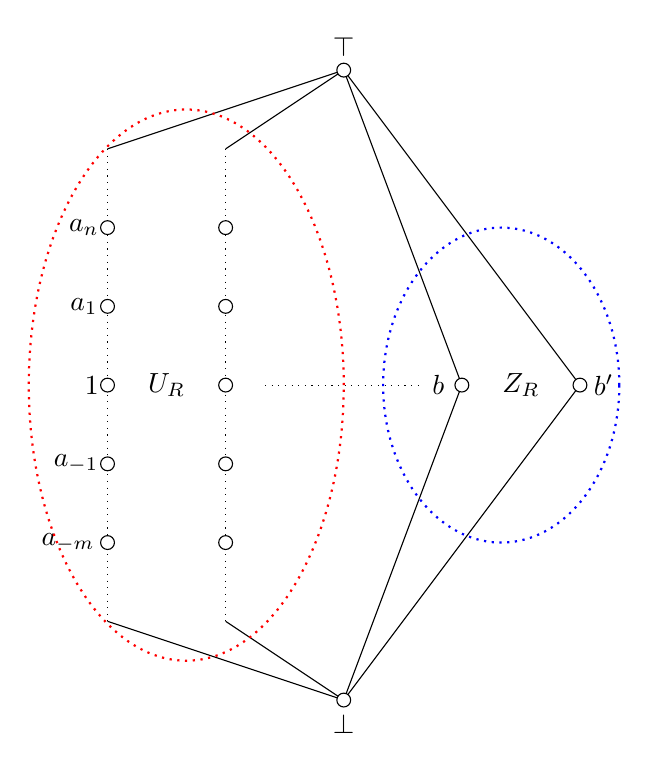
\begin{tikzpicture}
        \draw (3, 4) -- (0, 3);
        \draw[dotted] (0, 3) -- (0, -3);
        \draw (0, -3) -- (3, -4);
        \draw (3, 4) -- (1.5, 3);
        \draw[dotted] (1.5, 3) -- (1.5, -3);
        \draw (1.5, -3) -- (3, -4);
        \draw[dotted] (2, 0) -- (4, 0);
        \draw (3, 4) -- (4.5, 0) -- (3, -4);
        \draw (3, 4) -- (6, 0) -- (3, -4);

        \draw (0.75, 0) node {$U_R$};
        \draw (5.25, 0) node {$Z_R$};

        \filldraw [color = black, fill = white] (3, 4) circle (2.5pt)
            (3, 4.3) node {$\top$};
        \filldraw [color = black, fill = white] (3, -4) circle (2.5pt)
            (3, -4.3) node [black] {$\bot$};
        \filldraw [color = black, fill = white] (0, 2) circle (2.5pt)
            (-0.3, 2) node [black] {$a_n$};
        \filldraw [color = black, fill = white] (0, 1) circle (2.5pt)
            (-0.3, 1) node [black] {$a_1$};
        \filldraw [color = black, fill = white] (0, 0) circle (2.5pt)
            (-0.2, 0) node [black] {$1$};
        \filldraw [color = black, fill = white] (0, -1) circle (2.5pt)
            (-0.4, -1) node [black] {$a_{-1}$};
        \filldraw [color = black, fill = white] (0, -2) circle (2.5pt)
            (-0.5, -2) node [black] {$a_{-m}$};

        \filldraw [color = black, fill = white] (1.5, 2) circle (2.5pt);
        \filldraw [color = black, fill = white] (1.5, 1) circle (2.5pt);
        \filldraw [color = black, fill = white] (1.5, 0) circle (2.5pt);
        \filldraw [color = black, fill = white] (1.5, -1) circle (2.5pt);
        \filldraw [color = black, fill = white] (1.5, -2) circle (2.5pt);

        \filldraw [color = black, fill = white] (4.5, 0) circle (2.5pt)
            (4.2, 0) node [black] {$b$};
        \filldraw [color = black, fill = white] (6, 0) circle (2.5pt)
            (6.3, 0) node [black] {$b'$};

        \draw[red, thick, dotted] (1, 0) ellipse (2 and 3.5);
        \draw[blue, thick, dotted] (5, 0) ellipse (1.5 and 2);
        \end{tikzpicture}
        }
        \end{center}
    \end{columns}
\end{frame}

\begin{comment}
\begin{frame}{Construction of non-linear members of $\mathsf{B}$}
    \begin{figure}
    \centering
    \scalebox{0.6}{        
        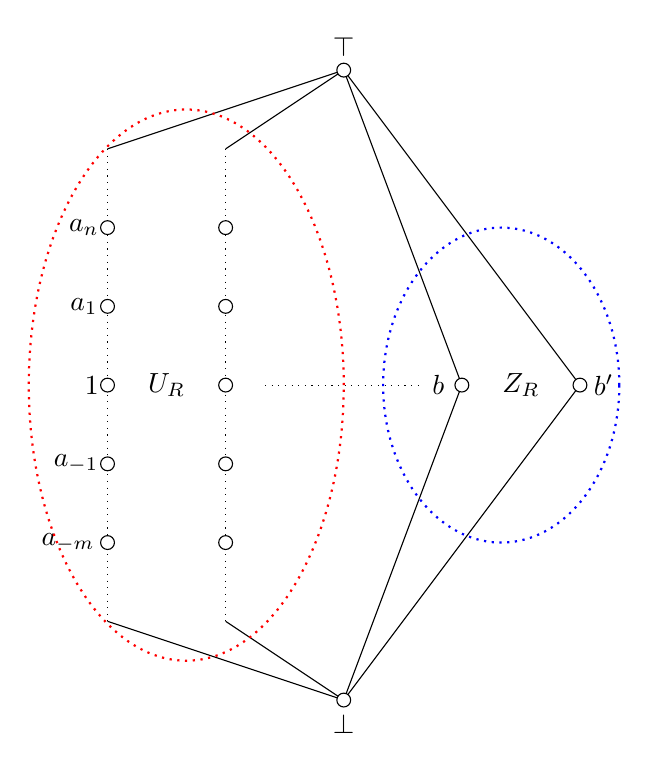
\begin{tikzpicture}
        \draw (3, 4) -- (0, 3);
        \draw[dotted] (0, 3) -- (0, -3);
        \draw (0, -3) -- (3, -4);
        \draw (3, 4) -- (1.5, 3);
        \draw[dotted] (1.5, 3) -- (1.5, -3);
        \draw (1.5, -3) -- (3, -4);
        \draw[dotted] (2, 0) -- (4, 0);
        \draw (3, 4) -- (4.5, 0) -- (3, -4);
        \draw (3, 4) -- (6, 0) -- (3, -4);

        \draw (0.75, 0) node {$U_R$};
        \draw (5.25, 0) node {$Z_R$};

        \filldraw [color = black, fill = white] (3, 4) circle (2.5pt)
            (3, 4.3) node {$\top$};
        \filldraw [color = black, fill = white] (3, -4) circle (2.5pt)
            (3, -4.3) node [black] {$\bot$};
        \filldraw [color = black, fill = white] (0, 2) circle (2.5pt)
            (-0.3, 2) node [black] {$a_n$};
        \filldraw [color = black, fill = white] (0, 1) circle (2.5pt)
            (-0.3, 1) node [black] {$a_1$};
        \filldraw [color = black, fill = white] (0, 0) circle (2.5pt)
            (-0.2, 0) node [black] {$1$};
        \filldraw [color = black, fill = white] (0, -1) circle (2.5pt)
            (-0.4, -1) node [black] {$a_{-1}$};
        \filldraw [color = black, fill = white] (0, -2) circle (2.5pt)
            (-0.5, -2) node [black] {$a_{-m}$};

        \filldraw [color = black, fill = white] (1.5, 2) circle (2.5pt);
        \filldraw [color = black, fill = white] (1.5, 1) circle (2.5pt);
        \filldraw [color = black, fill = white] (1.5, 0) circle (2.5pt);
        \filldraw [color = black, fill = white] (1.5, -1) circle (2.5pt);
        \filldraw [color = black, fill = white] (1.5, -2) circle (2.5pt);

        \filldraw [color = black, fill = white] (4.5, 0) circle (2.5pt)
            (4.2, 0) node [black] {$b$};
        \filldraw [color = black, fill = white] (6, 0) circle (2.5pt)
            (6.3, 0) node [black] {$b'$};

        \draw[red, thick, dotted] (1, 0) ellipse (2 and 3.5);
        \draw[blue, thick, dotted] (5, 0) ellipse (1.5 and 2);
        \end{tikzpicture}\pause
        \qquad
        \begin{tikzpicture}
        \draw (3.5, 4) -- (1, 3);
        \draw (1, -3) -- (3.5, -4);
        \draw (3.5, 4) -- (6, 3);
        \draw (6, -3) -- (3.5, -4);

        \draw (1, 0) node {$\mathbf{A}$};
        \draw[red, thick, dotted] (1, 0) ellipse (2 and 3);

        \draw (6, 0) node {$\mathbf{B}$};
        \draw[blue, thick, dotted] (6, 0) ellipse (2 and 3);

        \filldraw [color = black, fill = white] (3.5, 4) circle (2.5pt)
            (3.5, 4.4) node {$\top$};
        \filldraw [color = black, fill = white] (3.5, -4) circle (2.5pt)
            (3.5, -4.4) node [black] {$\bot$};
        \end{tikzpicture}
        }
    \caption{$\m R_{\m A, \m B}$}
    \end{figure}
\end{frame}
\end{comment}

\begin{comment}
\begin{frame}{Class $\mathsf{TW}$}
    In the class $\mathsf{TW}$, the non-linear members are axiomatized by
    \begin{align}
        & \forall x, y \, (x \leq y \text{ or } y \leq x \text{ or } x \backslash \bot \vee x = \top \text{ or } y \backslash \bot \vee y = \top) \tag{coml} \label{compl}\\
        & \forall x_1, x_2, x_3 \, (\bigor \limits_{1 \leq i \neq j \leq 3} x_i \leq x_j) \tag{$w_2$} \label{w2}
    \end{align}
    
\end{frame}

\begin{frame}{}
    \begin{figure}
    \centering
        \scalebox{0.6}{
            \begin{tikzpicture}
                \draw (2, 4) -- (0, 3);
                \draw[dotted] (0, 3) -- (0, -3);
                \draw (0, -3) -- (2, -4);
                \draw (2, 4) -- (4, 0) -- (2, -4);

                \filldraw [color = black, fill = white] (2, 4) circle (2.5pt)
                    (2, 4.3) node [black] {$\top$};
                \filldraw [color = black, fill = white] (2, -4) circle (2.5pt)
                    (2, -4.3) node [black] {$\bot$};
                \filldraw [color = black, fill = white] (0, 2) circle (2.5pt)
                    (-0.4, 2) node [black] {$a_n$};
                \filldraw [color = black, fill = white] (0, 1) circle (2.5pt)
                    (-0.4, 1) node [black] {$a_1$};
                \filldraw [color = black, fill = white] (0, 0) circle (2.5pt)
                    (-0.2, 0) node [black] {$1$};
                \filldraw [color = black, fill = white] (0, -1) circle (2.5pt)
                    (-0.5, -1) node [black] {$a_{-1}$};
                \filldraw [color = black, fill = white] (0, -2) circle (2.5pt)
                    (-0.5, -2) node [black] {$a_{-m}$};
                \filldraw [color = black, fill = white] (0, -3) circle (2.5pt)
                    (-0.3, -3) node [black] {$b$};
                \filldraw [color = black, fill = white] (4, 0) circle (2.5pt)
                    (4.3, 0) node [black] {$b'$};
            \end{tikzpicture}
            \begin{tikzpicture}
                \draw (2.5, 4) -- (0, 3);
                \draw[dotted] (0, 3) -- (0, -3);
                \draw (0, -3) -- (2.5, -4);
                \draw (2.5, 4) -- (5, 3);
                \draw[dotted] (5, 3) -- (5, -3);
                \draw (5, -3) -- (2.5, -4);

        \filldraw [color = black, fill = white] (2.5, 4) circle(2.5pt)
            (2.5, 4.4) node {$\top$};
        \filldraw [color = black, fill = white] (2.5, -4) circle(2.5pt)
            (2.5, -4.4) node {$\bot$};
        \filldraw [color = black, fill = white] (0, 2) circle(2.5pt)
            (-0.4, 2) node {$a_n$};
        \filldraw [color = black, fill = white] (0, 1) circle(2.5pt)
            (-0.4, 1) node {$a_1$};
        \filldraw [color = black, fill = white] (0, 0) circle(2.5pt)
            (-0.3, 0) node {$1$};
        \filldraw [color = black, fill = white] (0, -1) circle(2.5pt)
            (-0.4, -1) node {$a_{-1}$};
        \filldraw [color = black, fill = white] (0, -2) circle(2.5pt)
            (-0.5, -2) node {$a_{-m}$};
        \filldraw [color = black, fill = white] (0, -3) circle(2.5pt)
            (-0.3, -3) node {$b$};
            
        \filldraw [color = black, fill = white] (5, 3) circle(2.5pt)
            (5.4, 3) node {$b_0$};
        \filldraw [color = black, fill = white] (5, 2) circle(2.5pt)
            (5.4, 2) node {$c_n$};
        \filldraw [color = black, fill = white] (5, 1) circle(2.5pt);
        \filldraw [color = black, fill = white] (5, 0) circle(2.5pt)
            (5.4, 0) node {$c_0$};
        \filldraw [color = black, fill = white] (5, -1) circle(2.5pt);
        \filldraw [color = black, fill = white] (5, -2) circle(2.5pt)
            (5.5, -2) node {$c_{-m}$};
            \end{tikzpicture}
            }
    \caption{$\mathsf{TW}$: (a) $W = \emptyset$; (b) $W \neq \emptyset$}        
    \end{figure}
\end{frame}
\end{comment}

\begin{frame}{Class $\mathsf{TW}$}
    \begin{align}
        & \forall x, y \, (x \leq y \text{ or } y \leq x \text{ or } x \backslash \bot \vee x = \top \text{ or } y \backslash \bot \vee y = \top) \tag{coml} \label{compl}\\
        & \forall x_1, x_2, x_3 \, (\bigor \limits_{1 \leq i \neq j \leq 3} x_i \leq x_j) \tag{$w_2$} \label{w2}
    \end{align} \pause    
    \begin{figure}
    \centering
    \scalebox{0.5}{
    \begin{tikzpicture}
    \draw (2, 4) -- (0, 3);
    \draw[dotted] (0, 3) -- (0, -3);
    \draw (0, -3) -- (2, -4);
    \draw (2, 4) -- (4, 0) -- (2, -4);

    \filldraw [color = black, fill = white] (2, 4) circle (2.5pt)
    (2, 4.3) node [black] {$\top$};
    \filldraw [color = black, fill = white] (2, -4) circle (2.5pt)
    (2, -4.3) node [black] {$\bot$};
    \filldraw [color = black, fill = white] (0, 2) circle (2.5pt)
    (-0.4, 2) node [black] {$a_n$};
    \filldraw [color = black, fill = white] (0, 1) circle (2.5pt)
    (-0.4, 1) node [black] {$a_1$};
    \filldraw [color = black, fill = white] (0, 0) circle (2.5pt)
    (-0.2, 0) node [black] {$1$};
    \filldraw [color = black, fill = white] (0, -1) circle (2.5pt)
    (-0.5, -1) node [black] {$a_{-1}$};
    \filldraw [color = black, fill = white] (0, -2) circle (2.5pt)
    (-0.5, -2) node [black] {$a_{-m}$};
    \filldraw [color = black, fill = white] (0, -3) circle (2.5pt)
    (-0.3, -3) node [black] {$b$};
    \filldraw [color = black, fill = white] (4, 0) circle (2.5pt)
    (4.3, 0) node [black] {$b'$};

    \draw[thick, dotted, rotate around = {-15: (1, 0.5)}] (1, 0.5) ellipse (1.7 and 4);
    \end{tikzpicture}\pause
    \begin{tikzpicture}
        \draw (2.5, 4) -- (0, 3);
        \draw[dotted] (0, 3) -- (0, -3);
        \draw (0, -3) -- (2.5, -4);
        \draw (2.5, 4) -- (5, 3);
        \draw[dotted] (5, 3) -- (5, -3);
        \draw (5, -3) -- (2.5, -4);

        \draw[red, thick, dotted, rotate around = {-20: (1, 0.5)}] (1, 0.5) ellipse (1.6 and 4);
        \draw[blue, thick, dotted, rotate around = {-20: (4, -0.5)}] (4, -0.5) ellipse (1.6 and 4);

        \filldraw [color = black, fill = white] (2.5, 4) circle(2.5pt)
            (2.5, 4.4) node {$\top$};
        \filldraw [color = black, fill = white] (2.5, -4) circle(2.5pt)
            (2.5, -4.4) node {$\bot$};
        \filldraw [color = black, fill = white] (0, 2) circle(2.5pt)
            (-0.4, 2) node {$a_n$};
        \filldraw [color = black, fill = white] (0, 1) circle(2.5pt)
            (-0.4, 1) node {$a_1$};
        \filldraw [color = black, fill = white] (0, 0) circle(2.5pt)
            (-0.3, 0) node {$1$};
        \filldraw [color = black, fill = white] (0, -1) circle(2.5pt)
            (-0.4, -1) node {$a_{-1}$};
        \filldraw [color = black, fill = white] (0, -2) circle(2.5pt)
            (-0.5, -2) node {$a_{-m}$};
        \filldraw [color = black, fill = white] (0, -3) circle(2.5pt)
            (-0.3, -3) node {$b$};
            
        \filldraw [color = black, fill = white] (5, 3) circle(2.5pt)
            (5.4, 3) node {$b'$};
        \filldraw [color = black, fill = white] (5, 2) circle(2.5pt)
            (5.4, 2) node {$c_n$};
        \filldraw [color = black, fill = white] (5, 1) circle(2.5pt);
        \filldraw [color = black, fill = white] (5, 0) circle(2.5pt)
            (5.4, 0) node {$c_0$};
        \filldraw [color = black, fill = white] (5, -1) circle(2.5pt);
        \filldraw [color = black, fill = white] (5, -2) circle(2.5pt)
            (5.5, -2) node {$c_{-m}$};
        \end{tikzpicture}
    }
    %\caption{$\mathsf{TW}$: (a) $W = \emptyset$: $\m R_{\m A, \{b, b'\}}$; (b) $W \neq \emptyset$: $\m R_{\m A, \m C, *}$}
    \end{figure}
    
\end{frame}

\begin{comment}
\begin{frame}{Class $\mathsf{LW}$}
    The non-linear members in the class $\mathsf{LW}$ are axiomatized by
    \begin{equation}\tag{ZWlinear}\label{ZWlinear}
    \forall x, y \, (\top x = \top \text{ or } \top y = \top \text{ or } x \leq y \text{ or } y \leq x).
    \end{equation}
\end{frame}

\begin{frame}{}
    \begin{figure}
        \centering
        \scalebox{0.7}{
        \begin{tikzpicture}
        \draw (3, 4) -- (0, 3);
        \draw[dotted] (0, 3) -- (0, -3);
        \draw (0, -3) -- (3, -4);
        \draw (3, 4) -- (1.5, 3);
        \draw[dotted] (1.5, 3) -- (1.5, -3);
        \draw (1.5, -3) -- (3, -4);
        \draw[dotted] (2, 0) -- (5.5, 0);
        \draw (3, 4) -- (6, 3);
        \draw[dotted] (6, 3) -- (6, -3);
        \draw (6, -3) -- (3, -4);

        \filldraw [color = black, fill = white] (3, 4) circle (2.5pt)
            (3, 4.3) node {$\top$};
        \filldraw [color = black, fill = white] (3, -4) circle (2.5pt)
            (3, -4.3) node [black] {$\bot$};
        \filldraw [color = black, fill = white] (0, 2) circle (2.5pt)
            (-0.3, 2) node [black] {$a_n$};
        \filldraw [color = black, fill = white] (0, 1) circle (2.5pt)
            (-0.3, 1) node [black] {$a_1$};
        \filldraw [color = black, fill = white] (0, 0) circle (2.5pt)
            (-0.2, 0) node [black] {$1$};
        \filldraw [color = black, fill = white] (0, -1) circle (2.5pt)
            (-0.4, -1) node [black] {$a_{-1}$};
        \filldraw [color = black, fill = white] (0, -2) circle (2.5pt)
            (-0.5, -2) node [black] {$a_{-m}$};

        \filldraw [color = black, fill = white] (1.5, 2) circle (2.5pt);
        \filldraw [color = black, fill = white] (1.5, 1) circle (2.5pt);
        \filldraw [color = black, fill = white] (1.5, 0) circle (2.5pt)
            (1.3, 0) node {$a$};
        \filldraw [color = black, fill = white] (1.5, -1) circle (2.5pt);
        \filldraw [color = black, fill = white] (1.5, -2) circle (2.5pt);

        \filldraw [color = black, fill = white] (6, 2) circle (2.5pt)
            (6.3, 2) node {$b_1$};
        \filldraw [color = black, fill = white] (6, 1) circle (2.5pt);
        \filldraw [color = black, fill = white] (6, 0) circle (2.5pt);
        \filldraw [color = black, fill = white] (6, -1) circle (2.5pt);
        \filldraw [color = black, fill = white] (6, -2) circle (2.5pt)
            (6.3, -2) node {$b_i$};
        \end{tikzpicture}
        \qquad
        \begin{tikzpicture}
            \draw (3, 4) -- (0, 3);
        \draw[dotted] (0, 3) -- (0, -3);
        \draw (0, -3) -- (3, -4);
        \draw (3, 4) -- (1.5, 3);
        \draw[dotted] (1.5, 3) -- (1.5, -3);
        \draw (1.5, -3) -- (3, -4);
        \draw[dotted] (2, 0) -- (5.5, 0);
        \draw (3, 4) -- (6, 3);
        \draw[dotted] (6, 3) -- (6, -3);
        \draw (6, -3) -- (3, -4);

        \filldraw [color = black, fill = white] (3, 4) circle (2.5pt)
            (3, 4.3) node {$\top$};
        \filldraw [color = black, fill = white] (3, -4) circle (2.5pt)
            (3, -4.3) node {$\bot$};
        \filldraw [color = black, fill = white] (0, 2) circle (2.5pt)
            (-0.4, 2) node {$a_n$};
        \filldraw [color = black, fill = white] (0, 1) circle (2.5pt)
            (-0.4, 1) node {$a_1$};
        \filldraw [color = black, fill = white] (0, 0) circle (2.5pt)
            (-0.3, 0) node {$1$};
        \filldraw [color = black, fill = white] (0, -1) circle (2.5pt)
            (-0.5, -1) node {$a_{-1}$};
        \filldraw [color = black, fill = white] (0, -2) circle (2.5pt)
            (-0.5, -2) node {$a_{-m}$};

        \filldraw [color = black, fill = white] (1.5, 2) circle (2.5pt);
        \filldraw [color = black, fill = white] (1.5, 1) circle (2.5pt);
        \filldraw [color = black, fill = white] (1.5, 0) circle (2.5pt)
            (1.2, 0) node {$a$};
        \filldraw [color = black, fill = white] (1.5, -1) circle (2.5pt);
        \filldraw [color = black, fill = white] (1.5, -2) circle (2.5pt);

        \filldraw [color = black, fill = white] (6, 2) circle (2.5pt)
            (6.4, 2) node {$b_i$};
        \filldraw [color = black, fill = white] (6, 1) circle (2.5pt)
            (6.4, 1) node {$b_1$};
        \filldraw [color = black, fill = white] (6, 0) circle (2.5pt)
            (6.4, 0) node {$b_0$};
        \filldraw [color = black, fill = white] (6, -1) circle (2.5pt)
            (6.4, -1) node {$c_1$};
        \filldraw [color = black, fill = white] (6, -2) circle (2.5pt)
            (6.4, -2) node {$c_j$};
        \end{tikzpicture}
        }
        \caption{$\mathsf{LW}$: (a) $W = \emptyset$; (b) $W \neq \emptyset$}
    \end{figure}
\end{frame}
\end{comment}

\begin{frame}{Class $\mathsf{LW}$}

    \begin{equation}\tag{ZWlinear}\label{ZWlinear}
        \forall x, y \, (\top x = \top \text{ or } \top y = \top \text{ or } x \leq y \text{ or } y \leq x).
    \end{equation}
    \pause
    
    \begin{figure}
        \centering
        \scalebox{0.5}{
        \begin{tikzpicture}
        \draw (3, 4) -- (0, 3);
        \draw[dotted] (0, 3) -- (0, -3);
        \draw (0, -3) -- (3, -4);
        \draw (3, 4) -- (1.5, 3);
        \draw[dotted] (1.5, 3) -- (1.5, -3);
        \draw (1.5, -3) -- (3, -4);
        \draw[dotted] (2, 0) -- (5.5, 0);
        \draw (3, 4) -- (6, 3);
        \draw[dotted] (6, 3) -- (6, -3);
        \draw (6, -3) -- (3, -4);

        \draw[red, thick, dotted] (1, 0) ellipse (2 and 3.5);
        \draw[blue, thick, dotted] (6, 0) ellipse (2 and 3.5);

        \filldraw [color = black, fill = white] (3, 4) circle (2.5pt)
            (3, 4.3) node {$\top$};
        \filldraw [color = black, fill = white] (3, -4) circle (2.5pt)
            (3, -4.3) node [black] {$\bot$};
        \filldraw [color = black, fill = white] (0, 2) circle (2.5pt)
            (-0.3, 2) node [black] {$a_n$};
        \filldraw [color = black, fill = white] (0, 1) circle (2.5pt)
            (-0.3, 1) node [black] {$a_1$};
        \filldraw [color = black, fill = white] (0, 0) circle (2.5pt)
            (-0.2, 0) node [black] {$1$};
        \filldraw [color = black, fill = white] (0, -1) circle (2.5pt)
            (-0.4, -1) node [black] {$a_{-1}$};
        \filldraw [color = black, fill = white] (0, -2) circle (2.5pt)
            (-0.5, -2) node [black] {$a_{-m}$};

        \filldraw [color = black, fill = white] (1.5, 2) circle (2.5pt);
        \filldraw [color = black, fill = white] (1.5, 1) circle (2.5pt);
        \filldraw [color = black, fill = white] (1.5, 0) circle (2.5pt)
            (1.3, 0) node {$a$};
        \filldraw [color = black, fill = white] (1.5, -1) circle (2.5pt);
        \filldraw [color = black, fill = white] (1.5, -2) circle (2.5pt);

        \filldraw [color = black, fill = white] (6, 2) circle (2.5pt)
            (6.3, 2) node {$b_1$};
        \filldraw [color = black, fill = white] (6, 1) circle (2.5pt);
        \filldraw [color = black, fill = white] (6, 0) circle (2.5pt);
        \filldraw [color = black, fill = white] (6, -1) circle (2.5pt);
        \filldraw [color = black, fill = white] (6, -2) circle (2.5pt)
            (6.3, -2) node {$b_i$};
        \end{tikzpicture}\pause
        \qquad
        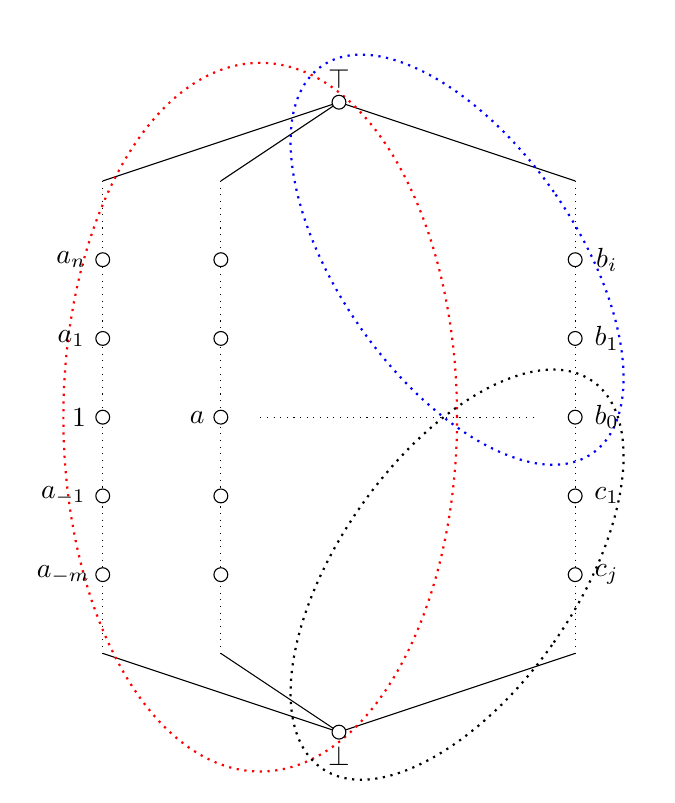
\begin{tikzpicture}
            \draw (3, 4) -- (0, 3);
        \draw[dotted] (0, 3) -- (0, -3);
        \draw (0, -3) -- (3, -4);
        \draw (3, 4) -- (1.5, 3);
        \draw[dotted] (1.5, 3) -- (1.5, -3);
        \draw (1.5, -3) -- (3, -4);
        \draw[dotted] (2, 0) -- (5.5, 0);
        \draw (3, 4) -- (6, 3);
        \draw[dotted] (6, 3) -- (6, -3);
        \draw (6, -3) -- (3, -4);

        \draw[red, thick, dotted] (2, 0) ellipse (2.5 and 4.5);
        \draw[blue, thick, dotted, rotate around = {35: (4.5, 2)}] (4.5, 2) ellipse (1.5 and 3);
        \draw[thick, dotted, rotate around = {-35: (4.5, -2)}] (4.5, -2) ellipse (1.5 and 3);

        \filldraw [color = black, fill = white] (3, 4) circle (2.5pt)
            (3, 4.3) node {$\top$};
        \filldraw [color = black, fill = white] (3, -4) circle (2.5pt)
            (3, -4.3) node {$\bot$};
        \filldraw [color = black, fill = white] (0, 2) circle (2.5pt)
            (-0.4, 2) node {$a_n$};
        \filldraw [color = black, fill = white] (0, 1) circle (2.5pt)
            (-0.4, 1) node {$a_1$};
        \filldraw [color = black, fill = white] (0, 0) circle (2.5pt)
            (-0.3, 0) node {$1$};
        \filldraw [color = black, fill = white] (0, -1) circle (2.5pt)
            (-0.5, -1) node {$a_{-1}$};
        \filldraw [color = black, fill = white] (0, -2) circle (2.5pt)
            (-0.5, -2) node {$a_{-m}$};

        \filldraw [color = black, fill = white] (1.5, 2) circle (2.5pt);
        \filldraw [color = black, fill = white] (1.5, 1) circle (2.5pt);
        \filldraw [color = black, fill = white] (1.5, 0) circle (2.5pt)
            (1.2, 0) node {$a$};
        \filldraw [color = black, fill = white] (1.5, -1) circle (2.5pt);
        \filldraw [color = black, fill = white] (1.5, -2) circle (2.5pt);

        \filldraw [color = black, fill = white] (6, 2) circle (2.5pt)
            (6.4, 2) node {$b_i$};
        \filldraw [color = black, fill = white] (6, 1) circle (2.5pt)
            (6.4, 1) node {$b_1$};
        \filldraw [color = black, fill = white] (6, 0) circle (2.5pt)
            (6.4, 0) node {$b_0$};
        \filldraw [color = black, fill = white] (6, -1) circle (2.5pt)
            (6.4, -1) node {$c_1$};
        \filldraw [color = black, fill = white] (6, -2) circle (2.5pt)
            (6.4, -2) node {$c_j$};
        \end{tikzpicture}
        }
        \caption{(a) $W = \emptyset$: $\m R_{\m A, \m B}$; (b) $W \neq \emptyset$: $\m R_{\m A, \m B, \m C, *}$}
    \end{figure}
\end{frame}

\begin{frame}{Class $\mathsf{B4}$}
\begin{columns}
    \column{0.5\textwidth}
    We denote the class of integral non-linear URLs by $\mathsf{B4}$.\pause

    $\mathsf{B4}$ is axiomatized by
    \[
        \forall x \, (\top x = x).
    \]
    \pause

    It turns out the only non-linear member in $\mathsf{B4}$ is the $4$-element Boolean algebra.\pause

    \column{0.5\textwidth}
    \begin{center}
    \scalebox{1}{
    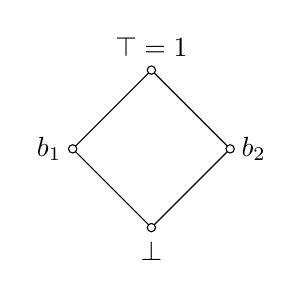
\begin{tikzpicture}
            \draw (1, 1) -- (0, 0) -- (1, -1);
            \draw (1, 1) -- (2, 0) -- (1, -1);

            \filldraw[color = black, fill = white] (1, 1) circle (1.5pt)
                (1, 1.3) node {$\top = 1$};
            \filldraw[color = black, fill = white] (1, -1) circle (1.5pt)
                (1, -1.3) node {$\bot$};
            \filldraw[color = black, fill = white] (0, 0) circle (1.5pt)
                (-0.3, 0) node {$b_1$};
            \filldraw[color = black, fill = white] (2, 0) circle (1.5pt)
                (2.3, 0) node {$b_2$};
        \end{tikzpicture}
        }
    \end{center}    
\end{columns}
\end{frame}

\begin{comment}
\begin{frame}{Characterization of URLs}
    \begin{block}{Theorem}
        Every URL belongs to one of the classes: $\mathsf{B}4$, $\top\mathsf{unital}$, $\mathsf{B}$, $\mathsf{TW}$, $\mathsf{LW}$.
        Moreover, the algebras in the last three classes can be constructed from algebras in the class $\top\mathsf{unital}$.
    \end{block}
\end{frame}
\end{comment}

\section{Applications}

\begin{frame}{URLs of type $h4.1$}
    We say a unilinear residuated lattice is of \emph{type} $h4.1$ if its lattice reduct is of the following form: all maximal chains have $3$ elements, except for one that has $4$ elements, as shown in the following diagram.
    \begin{center}
        \scalebox{0.7}{
        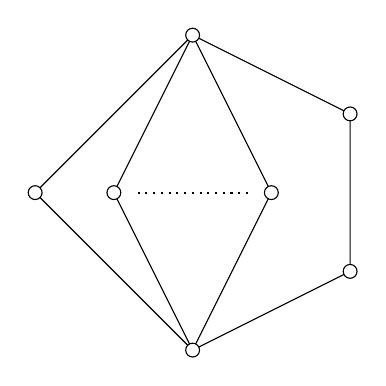
\begin{tikzpicture}
        \draw (2, 2) -- (0, 0) -- (2, -2);
        \draw (2, 2) -- (1, 0) -- (2, -2);
        \draw (2, 2) -- (3, 0) -- (2, -2);
        \draw (2, 2) -- (4, 1) -- (4, -1) -- (2, -2);
        \draw[thick, dotted] (1.3, 0) -- (2.7, 0);

        \filldraw[color = black, fill = white] (2, 2) circle(2.5pt);
        \filldraw[color = black, fill = white] (2, -2) circle(2.5pt);
        \filldraw[color = black, fill = white] (0, 0) circle(2.5pt);
        \filldraw[color = black, fill = white] (1, 0) circle(2.5pt);
        \filldraw[color = black, fill = white] (3, 0) circle(2.5pt);
        \filldraw[color = black, fill = white] (4, 1) circle(2.5pt);
        \filldraw[color = black, fill = white] (4, -1) circle(2.5pt);
        \end{tikzpicture}
        }
    \end{center}
\end{frame}

\begin{frame}{}
    \begin{figure}
    \centering
    \scalebox{0.5}{
    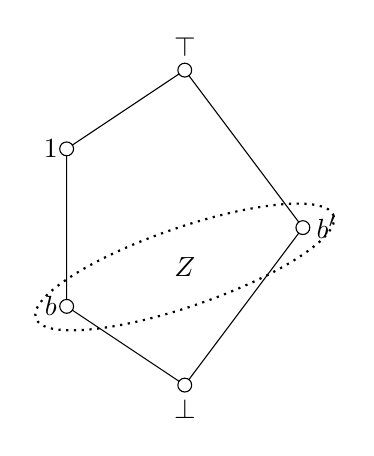
\begin{tikzpicture}
        \draw (1.5, 2) -- (0, 1) -- (0, -1) -- (1.5, -2);
        \draw (1.5, 2) -- (3, 0) -- (1.5, -2);

        \filldraw[color = black, fill = white] (1.5, 2) circle(2.5pt)
            (1.5, 2.3) node {$\top$};
        \filldraw[color = black, fill = white] (1.5, -2) circle(2.5pt)
            (1.5, -2.3) node {$\bot$};
        \filldraw[color = black, fill = white] (0, 1) circle(2.5pt)
            (-0.2, 1) node {$1$};
        \filldraw[color = black, fill = white] (0, -1) circle(2.5pt)
            (-0.2, -1) node {$b$};
        \filldraw[color = black, fill = white] (3, 0) circle(2.5pt)
            (3.3, 0) node {$b'$};

        \draw[thick, dotted, rotate around = {19: (1.5, -0.5)}] (1.5, -0.5) ellipse (2 and 0.5);
        \draw (1.5, -0.5) node {$Z$};
    \end{tikzpicture}
    \qquad
    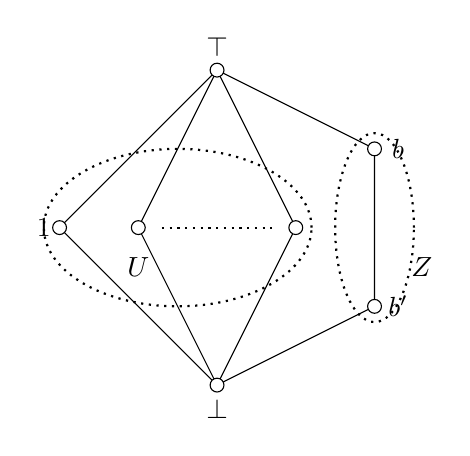
\begin{tikzpicture}
        \draw (2, 2) -- (0, 0) -- (2, -2);
        \draw (2, 2) -- (1, 0) -- (2, -2);
        \draw (2, 2) -- (3, 0) -- (2, -2);
        \draw (2, 2) -- (4, 1) -- (4, -1) -- (2, -2);
        \draw[thick, dotted] (1.3, 0) -- (2.7, 0);

        \filldraw[color = black, fill = white] (2, 2) circle(2.5pt)
            (2, 2.3) node {$\top$};
        \filldraw[color = black, fill = white] (2, -2) circle(2.5pt)
            (2, -2.3) node {$\bot$};
        \filldraw[color = black, fill = white] (0, 0) circle(2.5pt)
            (-0.2, 0) node {$1$};
        \filldraw[color = black, fill = white] (1, 0) circle(2.5pt);
        \filldraw[color = black, fill = white] (3, 0) circle(2.5pt);
        \filldraw[color = black, fill = white] (4, 1) circle(2.5pt)
            (4.3, 1) node {$b$};
        \filldraw[color = black, fill = white] (4, -1) circle(2.5pt)
            (4.3, -1) node {$b'$};

        \draw[thick, dotted] (1.5, 0) ellipse (1.7 and 1);
        \draw[thick, dotted] (4, 0) ellipse (0.5 and 1.2);

        \draw (1, -0.5) node {$U$};
        \draw (4.6, -0.5) node {$Z$};
    \end{tikzpicture}
    \qquad
    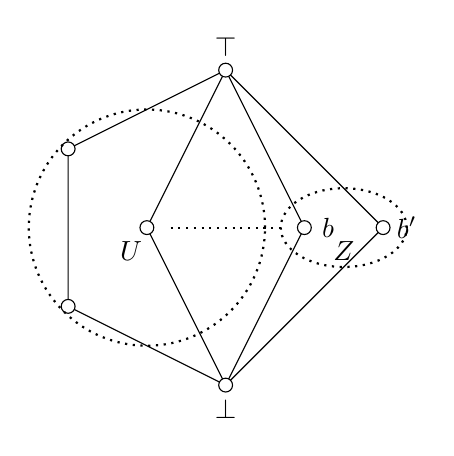
\begin{tikzpicture}
        \draw (2, 2) -- (0, 1) -- (0, -1) -- (2, -2);
        \draw (2, 2) -- (1, 0) -- (2, -2);
        \draw (2, 2) -- (3, 0) -- (2, -2);
        \draw (2, 2) -- (4, 0) -- (2, -2);
        \draw[thick, dotted] (1.3, 0) -- (2.7, 0);

        \filldraw[color = black, fill = white] (2, 2) circle(2.5pt)
            (2, 2.3) node {$\top$};
        \filldraw[color = black, fill = white] (2, -2) circle(2.5pt)
            (2, -2.3) node {$\bot$};
        \filldraw[color = black, fill = white] (0, 1) circle(2.5pt);
        \filldraw[color = black, fill = white] (0, -1) circle(2.5pt);
        \filldraw[color = black, fill = white] (1, 0) circle(2.5pt);
        \filldraw[color = black, fill = white] (3, 0) circle(2.5pt)
            (3.3, 0) node {$b$};
        \filldraw[color = black, fill = white] (4, 0) circle(2.5pt)
            (4.3, 0) node {$b'$};

        \draw[thick, dotted] (1, 0) ellipse (1.5 and 1.5);
        \draw[thick, dotted] (3.5, 0) ellipse (0.8 and 0.5);

        \draw (0.8, -0.3) node {$U$};
        \draw (3.5, -0.3) node {$Z$};
    \end{tikzpicture}
    }
    \scalebox{0.5}{
    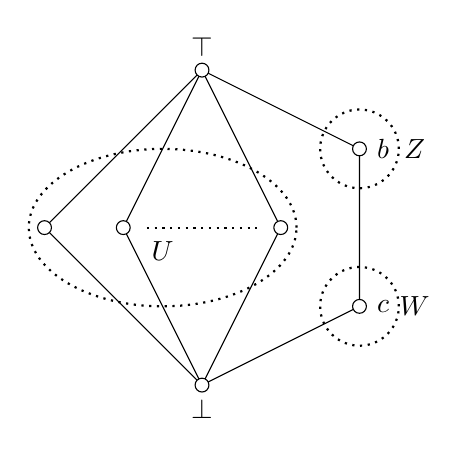
\begin{tikzpicture}
        \draw (2, 2) -- (0, 0) -- (2, -2);
        \draw (2, 2) -- (1, 0) -- (2, -2);
        \draw (2, 2) -- (3, 0) -- (2, -2);
        \draw (2, 2) -- (4, 1) -- (4, -1) -- (2, -2);
        \draw[thick, dotted] (1.3, 0) -- (2.7, 0);

        \filldraw[color = black, fill = white] (2, 2) circle(2.5pt)
            (2, 2.3) node {$\top$};
        \filldraw[color = black, fill = white] (2, -2) circle(2.5pt)
            (2, -2.3) node {$\bot$};
        \filldraw[color = black, fill = white] (0, 0) circle(2.5pt);
        \filldraw[color = black, fill = white] (1, 0) circle(2.5pt);
        \filldraw[color = black, fill = white] (3, 0) circle(2.5pt);
        \filldraw[color = black, fill = white] (4, 1) circle(2.5pt)
            (4.3, 1) node {$b$};
        \filldraw[color = black, fill = white] (4, -1) circle(2.5pt)
            (4.3, -1) node {$c$};

        \draw[thick, dotted] (1.5, 0) ellipse (1.7 and 1);
        \draw[thick, dotted] (4, 1) ellipse (0.5 and 0.5);
        \draw[thick, dotted] (4, -1) ellipse (0.5 and 0.5);

        \draw (1.5, -0.3) node {$U$};
        \draw (4.7, 1) node {$Z$};
        \draw (4.7, -1) node {$W$};
    \end{tikzpicture}
    \qquad
    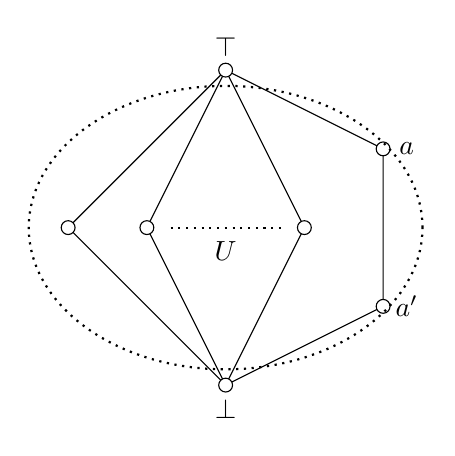
\begin{tikzpicture}
        \draw (2, 2) -- (0, 0) -- (2, -2);
        \draw (2, 2) -- (1, 0) -- (2, -2);
        \draw (2, 2) -- (3, 0) -- (2, -2);
        \draw (2, 2) -- (4, 1) -- (4, -1) -- (2, -2);
        \draw[thick, dotted] (1.3, 0) -- (2.7, 0);

        \filldraw[color = black, fill = white] (2, 2) circle(2.5pt)
            (2, 2.3) node {$\top$};
        \filldraw[color = black, fill = white] (2, -2) circle(2.5pt)
            (2, -2.3) node {$\bot$};
        \filldraw[color = black, fill = white] (0, 0) circle(2.5pt);
        \filldraw[color = black, fill = white] (1, 0) circle(2.5pt);
        \filldraw[color = black, fill = white] (3, 0) circle(2.5pt);
        \filldraw[color = black, fill = white] (4, 1) circle(2.5pt)
            (4.3, 1) node {$a$};
        \filldraw[color = black, fill = white] (4, -1) circle(2.5pt)
            (4.3, -1) node {$a'$};

        \draw[thick, dotted] (2, 0) ellipse (2.5 and 1.8);

        \draw (2, -0.3) node {$U$};
    \end{tikzpicture}
    }
\caption{Non-linear URLs type h4.1 are in $\mathsf{T}$, $\mathsf{L}$, $\mathsf{B}$, $\mathsf{LW}$ and $\top\mathsf{unital}$, respectively}
\end{figure}
\end{frame}

\begin{frame}{Idempotent URLs}
    A residuated lattice is called \emph{idempotent} if it satisfies
    \begin{equation}\tag{idem}\label{idempotent}
    \forall x \, (x^2 = x).
    \end{equation}
    \pause

    \begin{block}{Proposition}
        If $\m R$ is an idempotent non-linear unilinear residuated lattice, then $U_R$ is a subchain of the chain of $1$ and $W_R$ is empty.
    \end{block}
    \pause
    \medskip

    \begin{block}{Corollary}
        Every non-linear idempotent URL is either the $4$-element Boolean algebra, or it is contained in one of the classes $\mathsf{T}$, $\mathsf{B}$ and $\mathsf{L}$.
    \end{block}
\end{frame}

\begin{frame}{}
    \begin{figure}
    \centering
    \scalebox{0.6}{
    \begin{tikzpicture}
        \draw (1, 1) -- (0, 0) -- (1, -1);
        \draw (1, 1) -- (2, 0) -- (1, -1);

        \draw (1, -2) node {$\mathsf{B4}$};
            
        \filldraw[color = black, fill = white] (1, 1) circle (1.5pt)
            (1, 1.3) node {$\top$};
        \filldraw[color = black, fill = white] (1, -1) circle (1.5pt)
            (1, -1.3) node {$\bot$};
        \filldraw[color = black, fill = white] (0, 0) circle (1.5pt)
            (-0.3, 0) node {$b_1$};
        \filldraw[color = black, fill = white] (2, 0) circle (1.5pt)
            (2.3, 0) node {$b_2$};
    \end{tikzpicture}
    }
    \scalebox{0.5}{
    \begin{tikzpicture}
    \draw (2, 4) -- (0, 3);
    \draw[dotted] (0, 3) -- (0, 2) -- (0, 1) -- (0, 0) -- (0, -1) -- (0, -2) -- (0, -3);
    \draw (0, -3) -- (2, -4);
    \draw (2, 4) -- (4, 0) -- (2, -4);

    \draw (2, -4.9) node {$\mathsf{T}$};

    \filldraw [color = black, fill = white] (2, 4) circle (2.5pt)
    (2, 4.4) node [black] {$\top$};
    \filldraw [color = black, fill = white] (2, -4) circle (2.5pt)
    (2, -4.4) node [black] {$\bot$};
    \filldraw [color = black, fill = white] (0, 2) circle (2.5pt)
    (-0.3, 2) node [black] {$a_n$};
    \filldraw [color = black, fill = white] (0, 1) circle (2.5pt)
    (-0.3, 1) node [black] {$a_1$};
    \filldraw [color = black, fill = white] (0, 0) circle (2.5pt)
    (-0.3, 0) node [black] {$1$};
    \filldraw [color = black, fill = white] (0, -1) circle (2.5pt)
    (-0.4, -1) node [black] {$a_{-1}$};
    \filldraw [color = black, fill = white] (0, -2) circle (2.5pt)
    (-0.5, -2) node [black] {$a_{-m}$};
    \filldraw [color = black, fill = white] (0, -3) circle (2.5pt)
    (-0.3, -3) node [black] {$b$};
    \filldraw [color = black, fill = white] (4, 0) circle (2.5pt)
    (4.3, 0) node [black] {$b'$};
    \end{tikzpicture}
    \begin{tikzpicture}
        \draw (3, 4) -- (1, 3);
        \draw[dotted] (1, 3) -- (1, 2) -- (1, 1) -- (1, 0) -- (1, -1) -- (1, -2) -- (1, -3);
        \draw (1, -3) -- (3, -4);
        \draw (3, 4) -- (4.5, 0) -- (3, -4);
        \draw (3, 4) -- (6, 0) -- (3, -4);

        \draw (3, -4.9) node {$\mathsf{B}$};

        \filldraw [color = black, fill = white] (3, 4) circle (2.5pt)
            (3, 4.4) node {$\top$};
        \filldraw [color = black, fill = white] (3, -4) circle (2.5pt)
            (3, -4.4) node [black] {$\bot$};
        \filldraw [color = black, fill = white] (1, 2) circle (2.5pt)
            (0.7, 2) node [black] {$a_n$};
        \filldraw [color = black, fill = white] (1, 1) circle (2.5pt)
            (0.7, 1) node [black] {$a_1$};
        \filldraw [color = black, fill = white] (1, 0) circle (2.5pt)
            (0.7, 0) node [black] {$1$};
        \filldraw [color = black, fill = white] (1, -1) circle (2.5pt)
            (0.6, -1) node [black] {$a_{-1}$};
        \filldraw [color = black, fill = white] (1, -2) circle (2.5pt)
            (0.5, -2) node [black] {$a_{-m}$};
            
        \filldraw [color = black, fill = white] (4.5, 0) circle (2.5pt)
            (4.2, 0) node [black] {$b$};
        \filldraw [color = black, fill = white] (6, 0) circle (2.5pt)
            (6.3, 0) node [black] {$b'$};
    \end{tikzpicture}
    \begin{tikzpicture}
        \draw (2, 4) -- (0, 3);
        \draw[dotted] (0, 3) -- (0, 2) -- (0, 1) -- (0, 0) -- (0, -1) -- (0, -2) -- (0, -3);
        \draw (0, -3) -- (2, -4);
        \draw (2, 4) -- (4, 3);
        \draw[dotted] (4, 3) -- (4, 2) -- (4, 1) -- (4, -2) -- (4, -3);
        \draw (4, -3) -- (2, -4);

        \draw (2, -4.9) node {$\mathsf{L}$};

        \filldraw [color = black, fill = white] (2, 4) circle (2.5pt)
            (2, 4.4) node {$\top$};
        \filldraw [color = black, fill = white] (2, -4) circle (2.5pt)
            (2, -4.4) node [black] {$\bot$};
        \filldraw [color = black, fill = white] (0, 2) circle (2.5pt)
            (-0.3, 2) node [black] {$a_n$};
        \filldraw [color = black, fill = white] (0, 1) circle (2.5pt)
            (-0.3, 1) node [black] {$a_1$};
        \filldraw [color = black, fill = white] (0, 0) circle (2.5pt)
            (-0.3, 0) node [black] {$1$};
        \filldraw [color = black, fill = white] (0, -1) circle (2.5pt)
            (-0.5, -1) node [black] {$a_{-1}$};
        \filldraw [color = black, fill = white] (0, -2) circle (2.5pt)
            (-0.5, -2) node [black] {$a_{-m}$};

        \filldraw [color = black, fill = white] (4, 1) circle (2.5pt)
            (4.3, 1) node [black] {$b_i$};
        \filldraw [color = black, fill = white] (4, 0) circle (2.5pt);
        \filldraw [color = black, fill = white] (4, -1) circle (2.5pt)
            (4.3, -1) node [black] {$b_j$};
    \end{tikzpicture}
    }
        \caption{Non-linear idempotent URLs}
    \end{figure}
\end{frame}

\begin{frame}{Amalgamation property}
\begin{columns}
    \column{0.5\textwidth}
        \begin{figure}
        \centering
        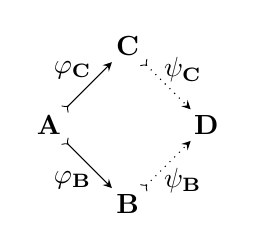
\begin{tikzpicture}
            \draw[>-stealth] (0.2, 0.2) -- (0.8, 0.8);
            \draw[>-stealth] (0.2, -0.2) -- (0.8, -0.8);
            \draw[dotted, >-stealth] (1.2, 0.8) -- (1.8, 0.2);
            \draw[dotted, >-stealth] (1.2, -0.8) -- (1.8, -0.2);

            \draw (0, 0) node {$\m A$};
            \draw (1, 1) node {$\m C$};
            \draw (1, -1) node {$\m B$};
            \draw (2, 0) node {$\m D$};

            \draw (0.3, 0.7) node {$\varphi_{\m C}$};
            \draw (0.3, -0.7) node {$\varphi_{\m B}$};
            \draw (1.7, 0.7) node {$\psi_{\m C}$};
            \draw (1.7, -0.7) node {$\psi_{\m B}$};
            
        \end{tikzpicture}
        \caption{AP and sAP}
    \end{figure}
    \pause

    \column{0.5\textwidth}

    $\psi_{\m B} \circ \varphi_{\m B} = \psi_{\m C} \circ \varphi_{\m C}$\pause
    \medskip

    $(\psi_{\m B} \circ \varphi_{\m B})[A] = \psi_{\m B}[B] \cap \psi_{\m C}[C]$
\end{columns}
\vspace{20pt}

By \cite{fussner2022conic}, the class of idempotent residuated chains fails AP, but the class of $\star$-involutive residuated chains has sAP.

\end{frame}

\begin{comment}
\begin{frame}{}
    We use $\mathsf{bURL}$ to denote the class of unilinear residuated lattices whose language contains constants $\bot$ and $\top$, which are evaluated as the bottom and top for the algebras.\pause
    Similarly, $\mathsf{bB4}$, $\mathsf{bT}$, $\mathsf{bB}$ and $\mathsf{bL}$ represent the subclasses of $\mathsf{bURL}$ axiomatized by the corresponding axioms.
    \medskip

    We use $\mathsf{B4_i}$ and $\mathsf{bB4_i}$ to denote the class of idempotent members in $\mathsf{B4}$ and $\mathsf{bB4}$.\pause
    \medskip

    $\mathsf{B4_i}$ and $\mathsf{bB4_i}$ fail amalgamation property.
\end{frame}
\end{comment}

\begin{frame}{}
    \begin{figure}
    \centering
    \scalebox{0.5}{
    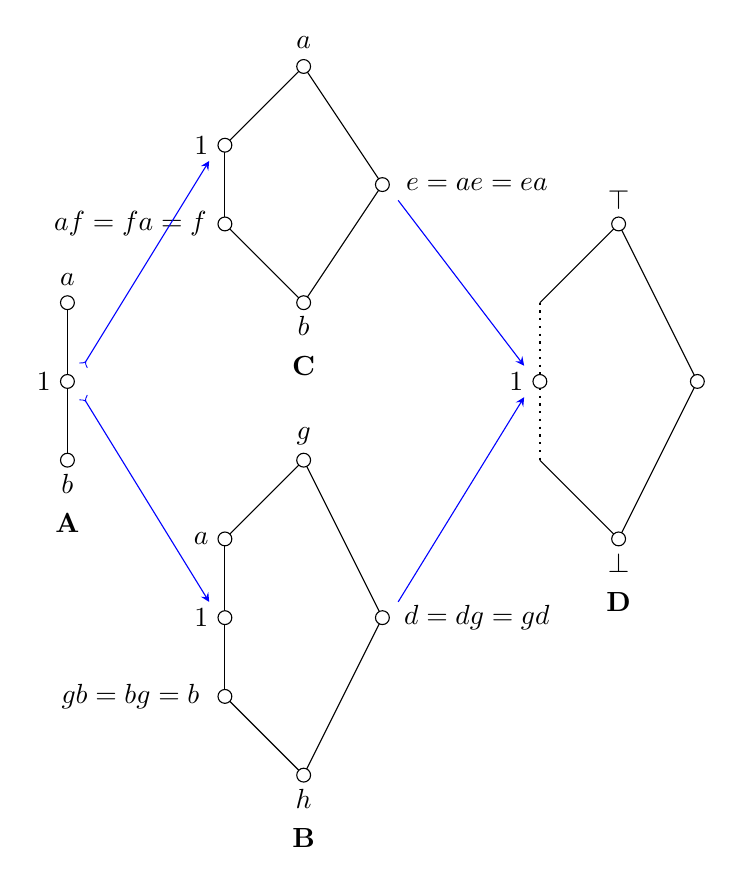
\begin{tikzpicture}
        \draw (0, 1) -- (0, -1);
        
        \draw (3, 4) -- (2, 3);
        \draw (2, 3) -- (2, 2);
        \draw (2, 2) -- (3, 1);
        \draw (3, 4) -- (4, 2.5) -- (3, 1);

        \draw (3, -1) -- (2, -2);
        \draw (2, -2) -- (2, -4);
        \draw (2, -4) -- (3, -5);
        \draw (3, -5) -- (4, -3) -- (3, -1);

        \draw (7, 2) -- (6, 1);
        \draw[thick, dotted] (6, 1) -- (6, -1);
        \draw (6, -1) -- (7, -2);
        \draw (7, 2) -- (8, 0) -- (7, -2);

        \filldraw[color = black, fill = white] (0, 1) circle(2.5pt)
            (0, 1.3) node {$a$};
        \filldraw[color = black, fill = white] (0, 0) circle(2.5pt)
            (-0.3, 0) node {$1$};
        \filldraw[color = black, fill = white] (0, -1) circle(2.5pt)
            (0, -1.3) node {$b$};
        
        \filldraw[color = black, fill = white] (3, 4) circle(2.5pt)
            (3, 4.3) node {$a$};
        \filldraw[color = black, fill = white] (2, 3) circle(2.5pt)
            (1.7, 3) node {$1$};
        \filldraw[color = black, fill = white] (2, 2) circle(2.5pt)
            (0.8, 2) node {$af = fa = f$};
        \filldraw[color = black, fill = white] (3, 1) circle(2.5pt)
            (3, 0.7) node {$b$};
        \filldraw[color = black, fill = white] (4, 2.5) circle(2.5pt)
            (5.2, 2.5) node {$e = ae = ea$};

        \filldraw[color = black, fill = white] (3, -1) circle(2.5pt)
            (3, -0.7) node {$g$};
        \filldraw[color = black, fill = white] (2, -2) circle(2.5pt)
            (1.7, -2) node {$a$};
        \filldraw[color = black, fill = white] (2, -3) circle(2.5pt)
            (1.7, -3) node {$1$};
        \filldraw[color = black, fill = white] (2, -4) circle(2.5pt)
            (0.8, -4) node {$gb = bg = b$};
        \filldraw[color = black, fill = white] (3, -5) circle(2.5pt)
            (3, -5.3) node {$h$};
        \filldraw[color = black, fill = white] (4, -3) circle(2.5pt)
            (5.2, -3) node {$d = dg = gd$};

        \filldraw[color = black, fill = white] (7, 2) circle(2.5pt)
            (7, 2.3) node {$\top$};
        \filldraw[color = black, fill = white] (6, 0) circle(2.5pt)
            (5.7, 0) node {$1$};
        \filldraw[color = black, fill = white] (7, -2) circle(2.5pt)
            (7, -2.3) node {$\bot$};
        \filldraw[color = black, fill = white] (8, 0) circle(2.5pt);

        \draw (0, -1.8) node {$\mathbf{A}$};
        \draw (3, 0.2) node {$\mathbf{C}$};
        \draw (3, -5.8) node {$\mathbf{B}$};
        \draw (7, -2.8) node {$\mathbf{D}$};

        \draw[blue, >-stealth] (0.2, 0.2) -- (1.8, 2.8);
        \draw[blue, >-stealth] (0.2, -0.2) -- (1.8, -2.8);
        \draw[blue, -stealth] (4.2, 2.3) -- (5.8, 0.2);
        \draw[blue, -stealth] (4.2, -2.8) -- (5.8, -0.2);
    \end{tikzpicture}
    }
    \pause
    \quad
    \scalebox{0.35}{
    \begin{tikzpicture}
        \draw[thick, dotted] (-1, 1) -- (-1, -1);
        \draw[thick, dotted] (2, 3) -- (2, 1);
        \draw[thick, dotted] (2, -1) -- (2, -3);
        \draw (2, -5) -- (1, -6);
        \draw[thick, dotted] (1, -6) -- (1, -8);
        \draw (1, -8) -- (2, -9);
        \draw (2, -5) -- (3, -7) -- (2, -9);
        \draw[thick, dotted] (5, 1) -- (5, -1);
        \draw (8, 2) -- (7, 1);
        \draw[thick, dotted] (7, 1) -- (7, -1);
        \draw (7, -1) -- (8, -2);
        \draw (8, 2) -- (9, 0) -- (8, -2);

        \draw (-4, 2) -- (-5, 1);
        \draw[thick, dotted] (-5, 1) -- (-5, -1);
        \draw (-5, -1) -- (-4, -2);
        \draw (-4, 2) -- (-3, 0) -- (-4, -2);

        \draw (2, 9) -- (1, 8);
        \draw[thick, dotted] (1, 8) -- (1, 6);
        \draw (1, 6) -- (2, 5);
        \draw (2, 9) -- (3, 7) -- (2, 5);

        \filldraw[color = black, fill = white] (-1, 1) circle(2.5pt)
            (-1, 1.3) node {$\top$};
        \filldraw[color = black, fill = white] (-1, 0) circle(2.5pt)
            (-0.7, 0) node {$1$};
        \filldraw[color = black, fill = white] (-1, -1) circle(2.5pt)
            (-1, -1.3) node {$b$};

        \filldraw[color = black, fill = white] (2, 3) circle(2.5pt)
            (2, 3.3) node {$\top$};
        \filldraw[color = black, fill = white] (2, 2) circle(2.5pt)
            (1.7, 2) node {$1$};
        \filldraw[color = black, fill = white] (2, 1) circle(2.5pt)
            (2, 0.7) node {$b$};

        \filldraw[color = black, fill = white] (2, -1) circle(2.5pt)
            (2, -0.7) node {$\top$};
        \filldraw[color = black, fill = white] (2, -2) circle(2.5pt)
            (1.7, -2) node {$1$};
        \filldraw[color = black, fill = white] (2, -3) circle(2.5pt)
            (2, -3.3) node {$b$};

        \filldraw[color = black, fill = white] (2, -5) circle(2.5pt)
            (2, -4.7) node {$\top$};
        \filldraw[color = black, fill = white] (1, -7) circle(2.5pt)
            (0.7, -7) node {$1$};
        \filldraw[color = black, fill = white] (1, -8) circle(2.5pt)
            (0.7, -8) node {$b$};
        \filldraw[color = black, fill = white] (2, -9) circle(2.5pt)
            (2, -9.3) node {$\bot$};
        \filldraw[color = black, fill = white] (3, -7) circle(2.5pt)
            (3.3, -7) node {$b'$};

        \filldraw[color = black, fill = white] (5, 1) circle(2.5pt)
            (5, 1.3) node {$\top$};
        \filldraw[color = black, fill = white] (5, 0) circle(2.5pt)
            (5.3, 0) node {$1$};
        \filldraw[color = black, fill = white] (5, -1) circle(2.5pt)
            (5, -1.3) node {$b$};

        \filldraw[color = black, fill = white] (8, 2) circle(2.5pt)
            (8, 2.3) node {$\top$};
        \filldraw[color = black, fill = white] (7, 0) circle(2.5pt)
            (6.7, 0) node {$1$};
        \filldraw[color = black, fill = white] (7, -1) circle(2.5pt)
            (6.7, -1) node {$b$};
        \filldraw[color = black, fill = white] (8, -2) circle(2.5pt)
            (8, -2.3) node {$\bot$};
        \filldraw[color = black, fill = white] (9, 0) circle(2.5pt)
            (9.3, 0) node {$b'$};

        \filldraw[color = black, fill = white] (-4, 2) circle(2.5pt)
            (-4, 2.3) node {$\top$};
        \filldraw[color = black, fill = white] (-5, 0) circle(2.5pt)
            (-5.3, 0) node {$1$};
        \filldraw[color = black, fill = white] (-5, -1) circle(2.5pt)
            (-5.3, -1) node {$b$};
        \filldraw[color = black, fill = white] (-4, -2) circle(2.5pt)
            (-4, -2.3) node {$\bot$};
        \filldraw[color = black, fill = white] (-3, 0) circle(2.5pt)
            (-2.7, 0) node {$b'$};

        \filldraw[color = black, fill = white] (2, 9) circle(2.5pt)
            (2, 9.3) node {$\top$};
        \filldraw[color = black, fill = white] (1, 7) circle(2.5pt)
            (0.7, 7) node {$1$};
        \filldraw[color = black, fill = white] (1, 6) circle(2.5pt)
            (0.7, 6) node {$b$};
        \filldraw[color = black, fill = white] (2, 5) circle(2.5pt)
            (2, 4.7) node {$\bot$};
        \filldraw[color = black, fill = white] (3, 7) circle(2.5pt)
            (3.3, 7) node {$b'$};

        \draw (-4, -2.8) node {$\mathbf{A} = \mathbf{B} \cap \mathbf{C}$};
        \draw (-1, -1.8) node {$\mathbf{A}'$};
        \draw (2, 4.2) node {$\mathbf{C}$};
        \draw (2, 0.2) node {$\mathbf{C}'$};
        \draw (2, -3.8) node {$\mathbf{B}'$};
        \draw (2, -9.8) node {$\mathbf{B}$};
        \draw (5, -1.8) node {$\mathbf{D}'$};
        \draw (8, -2.8) node {$\mathbf{D}$};

        \draw [blue, thick, -stealth] (-0.5, 0.2) -- (1.5, 2);
        \draw [blue, thick, -stealth] (2.3, 2) -- (4.8, 0.2);
        \draw [blue, thick, -stealth] (-0.5, -0.2) -- (1.5, -2);
        \draw [blue, thick, -stealth] (2, -4.5) -- (2, -4);
        \draw [blue, thick, -stealth] (2.3, -2) -- (4.8, -0.2);
        \draw [blue, thick, -stealth] (5.5, 0) -- (6.5, 0);
        \draw [blue, thick, -stealth] (-2.5, -0.2) -- (0.7, -6.5);
        \draw [blue, thick, -stealth] (-2.5, 0.2) -- (0.7, 6.5);
        \draw [blue, thick, -stealth] (3.5, -6.5) -- (6.5, -0.2);
        \draw [blue, thick, -stealth] (3.5, 6.5) -- (6.5, 0.2);
        \draw [blue, thick, -stealth] (-2.5, 0) -- (-1.3, 0);
        \draw [blue, thick, -stealth] (2, -4.5) -- (2, -4);
        \draw [blue, thick, -stealth] (2, 4) -- (2, 3.5);

        \draw (0.3, 1.3) node {$\varphi_C'$};
        \draw (-1.3, -3.5) node {$\varphi_B$};
        \draw (-1, 4) node {$\varphi_C$};
        \draw (0.3, -1.3) node {$\varphi_B'$};
        \draw (3.8, 1.3) node {$\psi_C'$};
        \draw (3.8, -1.3) node {$\psi_B'$};
        \draw (5.5, -3.5) node {$\psi_B$};
        \draw (5.5, 4) node {$\psi_C$};
    \end{tikzpicture}
    }
\caption{(a) Counterexample for AP of $\mathsf{T_i}$; (b) sAP of $\mathsf{bT_i}$}
\end{figure}

\end{frame}

\begin{frame}{$\star$-involution}
    Given a residuated lattice $\mathbf{R}$ and $x \in R$, we define
    \begin{align*}
    x^\ell = 1/x, \, x^r = x \backslash 1 \text{ and } x^{\star} = x^\ell \wedge x^r.
    \end{align*}
    $\m R$ is called \emph{$\star$-involutive} if $x^{\star \star} = x$ for all $x \in R$.\pause
    \vspace{20pt}

    Non-linear members in $\mathsf{T}$ and $\mathsf{L}$ are not $\star$-involutive.\pause

    \begin{equation}\tag{$\star$-inv${\updownarrow} 1$} \label{star_involutive}
    \forall x, y \, (x \leq y \text{ or } ((x \jn 1)^{\star \star} = x \jn 1 \text{ and } (x \mt 1)^{\star \star} = x \mt 1))
\end{equation}
\end{frame}

\begin{frame}{Congruence extension property and AP (sAP)}
    %By \cite{fussner2022transfer}, given an arithmetical variety $\mathcal{V}$ has the congruence extension property such that $\mathcal{V}_{FSI}$ is a universal class, if $\mathcal{V}_{FSI}$ has a strong amalgam in $\mathcal{V}$, then $\mathcal{V}$ has the strong amalgamation property.\pause
    %\medskip

    A class $\mathcal{K}$ has \emph{congruence extension property} (CEP) if for any $\m A \subseteq \m B \in \mathcal{K}$ and any $\theta \in \text{Con}(\m A)$, there is an $\eta \in \text{Con}(\m B)$ such that $\theta = \eta_{A \times A}$.\pause
    \medskip

    \begin{block}{Theorem}
        The varieties $\mathsf{IdSRL}$ and $\mathsf{bIdSRL}$ have the congruence extension property.
    \end{block}
    \pause
    \medskip
    
    \begin{figure}
    \centering
    \scalebox{0.6}{
    \begin{tabular}{c|c|c|c|c}
         & $\mathsf{T_i}$ & $\mathsf{bT_i}$ & $\mathsf{V(T_i)}$ & $\mathsf{V(bT_i)}$\\
        \hline
        AP & \xmark & \cmark & \xmark & \cmark\\
        \hline
        sAP & \xmark & \cmark & \xmark & \cmark
    \end{tabular}
    \qquad
    \begin{tabular}{c|c|c|c|c}
         & $\mathsf{B_i}$ & $\mathsf{bB_i}$ & $\mathsf{V(B_i)}$ & $\mathsf{V(bB_i)}$\\
        \hline
        AP & \xmark & \cmark & \xmark & ?\\
        \hline
        sAP & \xmark & \xmark & \xmark & ?
    \end{tabular}
    \qquad
    \begin{tabular}{c|c|c|c|c}
         & $\mathsf{L_i}$ & $\mathsf{bL_i}$ & $\mathsf{V(L_i)}$ & $\mathsf{V(bL_i)}$\\
        \hline
        AP & \xmark & \cmark & \xmark & \cmark\\
        \hline
        sAP & \xmark & \cmark & \xmark & \cmark
    \end{tabular}
    }
    \caption{AP and sAP for classes and varieties}
\end{figure}
\end{frame}

\begin{comment}
\begin{frame}{AP and sAP for classes and varieties}
\begin{figure}
    \centering
    \scalebox{0.6}{
    \begin{tabular}{c|c|c|c|c}
         & $\mathsf{T_i}$ & $\mathsf{bT_i}$ & $\mathsf{V(T_i)}$ & $\mathsf{V(bT_i)}$\\
        \hline
        AP & \xmark & \cmark & \xmark & \cmark\\
        \hline
        sAP & \xmark & \cmark & \xmark & \cmark
    \end{tabular}
    \qquad
    \begin{tabular}{c|c|c|c|c}
         & $\mathsf{B_i}$ & $\mathsf{bB_i}$ & $\mathsf{V(B_i)}$ & $\mathsf{V(bB_i)}$\\
        \hline
        AP & \xmark & \cmark & \xmark & ?\\
        \hline
        sAP & \xmark & \xmark & \xmark & ?
    \end{tabular}
    \qquad
    \begin{tabular}{c|c|c|c|c}
         & $\mathsf{L_i}$ & $\mathsf{bL_i}$ & $\mathsf{V(L_i)}$ & $\mathsf{V(bL_i)}$\\
        \hline
        AP & \xmark & \cmark & \xmark & \cmark\\
        \hline
        sAP & \xmark & \cmark & \xmark & \cmark
    \end{tabular}
    }
    \caption{AP and sAP for classes and varieties}
\end{figure}
\end{frame}
\end{comment}

\begin{frame}{AP for joins of varieties}
    \begin{block}{Theorem}
    The joins of any two of the varieties $\mathsf{V(bT_i)}$, $\mathsf{V(bB_i)}$ and $\mathsf{V(bL_i)}$ fail amalgamation property.
    \end{block}
    \pause

\begin{columns}
    \column{0.5\textwidth}
    Proof idea: By \cite{fussner2022transfer}, we show any join fails \emph{one-side amalgamation property}.\pause

    \column{0.5\textwidth}
    \begin{figure}
        \centering
        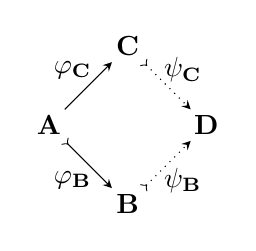
\begin{tikzpicture}
            \draw[-stealth] (0.2, 0.2) -- (0.8, 0.8);
            \draw[>-stealth] (0.2, -0.2) -- (0.8, -0.8);
            \draw[dotted, >-stealth] (1.2, 0.8) -- (1.8, 0.2);
            \draw[dotted, >-stealth] (1.2, -0.8) -- (1.8, -0.2);

            \draw (0, 0) node {$\m A$};
            \draw (1, 1) node {$\m C$};
            \draw (1, -1) node {$\m B$};
            \draw (2, 0) node {$\m D$};

            \draw (0.3, 0.7) node {$\varphi_{\m C}$};
            \draw (0.3, -0.7) node {$\varphi_{\m B}$};
            \draw (1.7, 0.7) node {$\psi_{\m C}$};
            \draw (1.7, -0.7) node {$\psi_{\m B}$};
            
        \end{tikzpicture}
        \caption{1AP}
    \end{figure}
\end{columns}
    
\end{frame}

\begin{frame}{$1$-involutive URL}
    Given a residuated lattice $\m R$ and $x \in R$.
    Recall
    \[
        x^\ell = 1/x \text{ and } x^r = x \ld 1.
    \]
    $\m R$ is called \emph{$1$-involutive} if it satisfies $x^{\ell r} = x = x^{r \ell}$ for all $x \in R$.
    
    %\begin{block}{Theorem}
        %Here are all the commutative $1$-involutive URL: the $\top$-unital ones; the non-$\top$-unital ones in the class $\mathsf{LW}$ in which $W = \emptyset$, $Z \cup \{\bot, \top\}$ is an integral residuated chain, such that $\top$-unital subalgebra is $1$-involutive and the $1$-free subalgebra $Z \cup \{\bot, \top\}$ is $\bot$-involutive; the ones in $\mathsf{B}$ whose $\top$-unital subalgebra is $1$-involutive.
    %\end{block}
\end{frame}

\begin{frame}{}
    \begin{figure}
        \centering
        \scalebox{0.5}{
        \begin{tikzpicture}
        \draw (3, 4) -- (0, 3);
        \draw[dotted] (0, 3) -- (0, -3);
        \draw (0, -3) -- (3, -4);
        \draw (3, 4) -- (1.5, 3);
        \draw[dotted] (1.5, 3) -- (1.5, -3);
        \draw (1.5, -3) -- (3, -4);
        \draw[dotted] (2, 0) -- (5.5, 0);
        \draw (3, 4) -- (6, 3);
        \draw[dotted] (6, 3) -- (6, -3);
        \draw (6, -3) -- (3, -4);

        \draw (3, -5) node {$\mathsf{Tunital}$};

        \filldraw [color = black, fill = white] (3, 4) circle (2.5pt)
            (3, 4.4) node {$\top$};
        \filldraw [color = black, fill = white] (3, -4) circle (2.5pt)
            (3, -4.4) node [black] {$\bot$};
        \filldraw [color = black, fill = white] (0, 2) circle (2.5pt)
            (-0.3, 2.3) node [black] {};
        \filldraw [color = black, fill = white] (0, 1) circle (2.5pt)
            (-0.3, 1.3) node [black] {};
        \filldraw [color = black, fill = white] (0, 0) circle (2.5pt)
            (-0.3, 0.3) node [black] {};
        \filldraw [color = black, fill = white] (0, -1) circle (2.5pt)
            (-0.4, -0.7) node [black] {};
        \filldraw [color = black, fill = white] (0, -2) circle (2.5pt)
            (-0.4, -1.7) node [black] {};

        \filldraw [color = black, fill = white] (1.5, 2) circle (2.5pt);
        \filldraw [color = black, fill = white] (1.5, 1) circle (2.5pt);
        \filldraw [color = black, fill = white] (1.5, 0) circle (2.5pt)
            (1.2, 0.3) node {};
        \filldraw [color = black, fill = white] (1.5, -1) circle (2.5pt);
        \filldraw [color = black, fill = white] (1.5, -2) circle (2.5pt);

        \filldraw [color = black, fill = white] (6, 2) circle (2.5pt);
        \filldraw [color = black, fill = white] (6, 1) circle (2.5pt);
        \filldraw [color = black, fill = white] (6, 0) circle (2.5pt)
            (6.3, 0.3) node [black] {};
        \filldraw [color = black, fill = white] (6, -1) circle (2.5pt);
        \filldraw [color = black, fill = white] (6, -2) circle (2.5pt);
        \end{tikzpicture}
        \begin{tikzpicture}
        \draw (3, 4) -- (0, 3);
        \draw[dotted] (0, 3) -- (0, -3);
        \draw (0, -3) -- (3, -4);
        \draw (3, 4) -- (1.5, 3);
        \draw[dotted] (1.5, 3) -- (1.5, -3);
        \draw (1.5, -3) -- (3, -4);
        \draw[dotted] (2, 0) -- (4, 0);
        \draw (3, 4) -- (4.5, 0) -- (3, -4);
        \draw (3, 4) -- (6, 0) -- (3, -4);

        \draw (3, -5) node {$\mathsf{B}$};

        \filldraw [color = black, fill = white] (3, 4) circle (2.5pt)
            (3, 4.3) node {$\top$};
        \filldraw [color = black, fill = white] (3, -4) circle (2.5pt)
            (3, -4.3) node [black] {$\bot$};
        \filldraw [color = black, fill = white] (0, 2) circle (2.5pt)
            (-0.3, 2) node [black] {$a_n$};
        \filldraw [color = black, fill = white] (0, 1) circle (2.5pt)
            (-0.3, 1) node [black] {$a_1$};
        \filldraw [color = black, fill = white] (0, 0) circle (2.5pt)
            (-0.2, 0) node [black] {$1$};
        \filldraw [color = black, fill = white] (0, -1) circle (2.5pt)
            (-0.4, -1) node [black] {$a_{-1}$};
        \filldraw [color = black, fill = white] (0, -2) circle (2.5pt)
            (-0.5, -2) node [black] {$a_{-m}$};

        \filldraw [color = black, fill = white] (1.5, 2) circle (2.5pt);
        \filldraw [color = black, fill = white] (1.5, 1) circle (2.5pt);
        \filldraw [color = black, fill = white] (1.5, 0) circle (2.5pt);
        \filldraw [color = black, fill = white] (1.5, -1) circle (2.5pt);
        \filldraw [color = black, fill = white] (1.5, -2) circle (2.5pt);

        \filldraw [color = black, fill = white] (4.5, 0) circle (2.5pt)
            (4.2, 0) node [black] {$b$};
        \filldraw [color = black, fill = white] (6, 0) circle (2.5pt)
            (6.3, 0) node [black] {$b'$};
        \end{tikzpicture}
        \begin{tikzpicture}
        \draw (3, 4) -- (0, 3);
        \draw[dotted] (0, 3) -- (0, -3);
        \draw (0, -3) -- (3, -4);
        \draw (3, 4) -- (1.5, 3);
        \draw[dotted] (1.5, 3) -- (1.5, -3);
        \draw (1.5, -3) -- (3, -4);
        \draw[dotted] (2, 0) -- (5.5, 0);
        \draw (3, 4) -- (6, 3);
        \draw[dotted] (6, 3) -- (6, -3);
        \draw (6, -3) -- (3, -4);

        \draw (3, -5) node {$\mathsf{L}$};

        \filldraw [color = black, fill = white] (3, 4) circle (2.5pt)
            (3, 4.3) node {$\top$};
        \filldraw [color = black, fill = white] (3, -4) circle (2.5pt)
            (3, -4.3) node [black] {$\bot$};
        \filldraw [color = black, fill = white] (0, 2) circle (2.5pt)
            (-0.3, 2) node [black] {$a_n$};
        \filldraw [color = black, fill = white] (0, 1) circle (2.5pt)
            (-0.3, 1) node [black] {$a_1$};
        \filldraw [color = black, fill = white] (0, 0) circle (2.5pt)
            (-0.2, 0) node [black] {$1$};
        \filldraw [color = black, fill = white] (0, -1) circle (2.5pt)
            (-0.4, -1) node [black] {$a_{-1}$};
        \filldraw [color = black, fill = white] (0, -2) circle (2.5pt)
            (-0.5, -2) node [black] {$a_{-m}$};

        \filldraw [color = black, fill = white] (1.5, 2) circle (2.5pt);
        \filldraw [color = black, fill = white] (1.5, 1) circle (2.5pt);
        \filldraw [color = black, fill = white] (1.5, 0) circle (2.5pt)
            (1.3, 0) node {$a$};
        \filldraw [color = black, fill = white] (1.5, -1) circle (2.5pt);
        \filldraw [color = black, fill = white] (1.5, -2) circle (2.5pt);

        \filldraw [color = black, fill = white] (6, 2) circle (2.5pt)
            (6.3, 2) node {$b_1$};
        \filldraw [color = black, fill = white] (6, 1) circle (2.5pt);
        \filldraw [color = black, fill = white] (6, 0) circle (2.5pt);
        \filldraw [color = black, fill = white] (6, -1) circle (2.5pt);
        \filldraw [color = black, fill = white] (6, -2) circle (2.5pt)
            (6.3, -2) node {$b_i$};
        \end{tikzpicture}
        }
        \caption{Non-linear commutative $1$-involutive URLs: (a) $\top$-unital;\\
        (b) $U \cup \{\bot, \top\}$ is $1$-involutive;\\
        (c) $U \cup \{\bot, \top\}$ is $1$-involutive and $Z \cup \{\bot, \top\}$ is $\bot$-involutive}
    \end{figure}
\end{frame}

\begin{frame}{Commutative $1$-involutive $\top$-unital URLs}
\begin{columns}
    \column{0.5\textwidth}
    Given a $1$-involutive residuated chain $\m H$ and a group $\m G$, we can define a $1$-involutive URL on $H \times G$, denoted as $\m H \times^b \m G$.
    \pause

    \column{0.5\textwidth}
    \begin{figure}
        \centering
        \scalebox{0.55}{
        \begin{tikzpicture}
        \draw (3, 4) -- (0, 3);
        \draw[dotted] (0, 3) -- (0, -3);
        \draw (0, -3) -- (3, -4);
        \draw (3, 4) -- (1.5, 3);
        \draw[dotted] (1.5, 3) -- (1.5, -3);
        \draw (1.5, -3) -- (3, -4);
        \draw[dotted] (2, 0) -- (4, 0);
        \draw (3, 4) -- (4.5, 3);
        \draw[dotted] (4.5, 3) -- (4.5, -3);
        \draw (4.5, -3) -- (3, -4);
        \draw (3, 4) -- (6, 3);
        \draw[dotted] (6, 3) -- (6, -3);
        \draw (6, -3) -- (3, -4);

        \filldraw [color = black, fill = white] (3, 4) circle (2.5pt)
            (3, 4.4) node {$\top$};
        \filldraw [color = black, fill = white] (3, -4) circle (2.5pt)
            (3, -4.4) node [black] {$\bot$};
        \filldraw [color = black, fill = white] (0, 2) circle (2.5pt);
        \filldraw [color = black, fill = white] (0, 1) circle (2.5pt);
        \filldraw [color = black, fill = white] (0, 0) circle (2.5pt)
            (-0.3, 0) node {$1$};
        \filldraw [color = black, fill = white] (0, -1) circle (2.5pt);
        \filldraw [color = black, fill = white] (0, -2) circle (2.5pt);

        \filldraw [color = black, fill = white] (1.5, 2) circle (2.5pt);
        \filldraw [color = black, fill = white] (1.5, 1) circle (2.5pt);
        \filldraw [color = black, fill = white] (1.5, 0) circle (2.5pt);
        \filldraw [color = black, fill = white] (1.5, -1) circle (2.5pt);
        \filldraw [color = black, fill = white] (1.5, -2) circle (2.5pt);

        \filldraw [color = black, fill = white] (4.5, 2) circle (2.5pt);
        \filldraw [color = black, fill = white] (4.5, 1) circle (2.5pt);
        \filldraw [color = black, fill = white] (4.5, 0) circle (2.5pt);
        \filldraw [color = black, fill = white] (4.5, -1) circle (2.5pt);
        \filldraw [color = black, fill = white] (4.5, -2) circle (2.5pt);

        \filldraw [color = black, fill = white] (6, 2) circle (2.5pt);
        \filldraw [color = black, fill = white] (6, 1) circle (2.5pt);
        \filldraw [color = black, fill = white] (6, 0) circle (2.5pt);
        \filldraw [color = black, fill = white] (6, -1) circle (2.5pt);
        \filldraw [color = black, fill = white] (6, -2) circle (2.5pt);
        \end{tikzpicture}
        }
        \caption{$\m H \times^b \m G$}
    \end{figure}
\end{columns}
    
\end{frame}

\begin{frame}{}
    A residuated chain $\m H$ is an \emph{odd Sugihara chain} if it satisfies commutativity, idempotency and $1$-involution.\pause
    \medskip

    An operator $\sigma$ on a residuated lattice $\m R$ is called a \emph{conucleus} if it is contracting ($\sigma(x) \leq x$), monotone ($x \leq y \implies \sigma(x) \leq \sigma(y)$), idempotent ($\sigma(\sigma(x)) = \sigma(x)$) and satisfies $\sigma(x) \sigma(1) = \sigma(1) \sigma(x) = \sigma(x)$ and $\sigma(x) \sigma(y) \leq \sigma(xy)$.
    \pause
    \medskip

    \begin{block}{Theorem}
        If $\m H$ is an odd Sugihara chain, $\m G$ is an abelian group whose elements are of finite orders and $\sigma$ is a conucleus on $ \m H \times^b \m G$ such that $\sigma$ is the identity on $(H \times \{1\}) \cup \{\bot, \top\}$, then $\sigma[\m H \times^b \m G]$ is a commutative $1$-involutive $\top$-unital URL.
    \end{block}
\end{frame}

\begin{frame}{}
\begin{figure}
    \centering
    \scalebox{0.5}{
    \begin{tikzpicture}
        \draw (3, 4) -- (0, 3);
        \draw[dotted] (0, 3) -- (0, 2);
        \draw (0, 2) -- (0, -2);
        \draw[dotted] (0, -2) -- (0, -3);
        \draw (0, -3) -- (3, -4);
        \draw (3, 4) -- (1.5, 3);
        \draw[dotted] (1.5, 3) -- (1.5, 2);
        \draw (1.5, 2) -- (1.5, -2);
        \draw[dotted] (1.5, -2) -- (1.5, -3);
        \draw (1.5, -3) -- (3, -4);
        \draw (3, 4) -- (4.5, 3);
        \draw[dotted] (4.5, 3) -- (4.5, 2);
        \draw (4.5, 2) -- (4.5, -2);
        \draw[dotted] (4.5, -2) -- (4.5, -3);
        \draw (4.5, -3) -- (3, -4);
        \draw (3, 4) -- (6, 3);
        \draw[dotted] (6, 3) -- (6, 2);
        \draw (6, 2) -- (6, -2);
        \draw[dotted] (6, -2) -- (6, -3);
        \draw (6, -3) -- (3, -4);

        \draw[dotted] (2, 0) -- (4, 0);

        \filldraw (3, 4) circle (2.5pt)
            (3, 4.4) node {$\top$};
        \filldraw (3, -4) circle (2.5pt)
            (3, -4.4) node [black] {$\bot$};
        \filldraw (0, 2) circle (2.5pt);
        \filldraw (0, 1) circle (2.5pt);
        \filldraw (0, 0) circle (2.5pt)
            (-0.3, 0) node {$1$};
        \filldraw (0, -1) circle (2.5pt);
        \filldraw (0, -2) circle (2.5pt);

        \filldraw (1.5, 2) circle (2.5pt);
        \filldraw (1.5, 1) circle (2.5pt);
        \filldraw (1.5, 0) circle (2.5pt);
        \filldraw (1.5, -1) circle (2.5pt);
        \filldraw (1.5, -2) circle (2.5pt);

        \filldraw (4.5, 2) circle (2.5pt);
        \filldraw (4.5, 1) circle (2.5pt);
        \filldraw (4.5, 0) circle (2.5pt);
        \filldraw (4.5, -1) circle (2.5pt);
        \filldraw (4.5, -2) circle (2.5pt);

        \filldraw (6, 2) circle (2.5pt);
        \filldraw (6, 1) circle (2.5pt);
        \filldraw (6, 0) circle (2.5pt);
        \filldraw (6, -1) circle (2.5pt);
        \filldraw (6, -2) circle (2.5pt);
    \end{tikzpicture}
    \qquad
    \begin{tikzpicture}
        \draw (3, 4) -- (0, 3);
        \draw[dotted] (0, 3) -- (0, 2);
        \draw (0, 2) -- (0, -2);
        \draw[dotted] (0, -2) -- (0, -3);
        \draw (0, -3) -- (3, -4);
        \draw (3, 4) -- (1.5, 3);
        \draw[dotted] (1.5, 3) -- (1.5, 2);
        \draw[dotted] (1.5, -2) -- (1.5, -3);
        \draw (1.5, -3) -- (3, -4);
        \draw (3, 4) -- (4.5, 3);
        \draw[dotted] (4.5, 3) -- (4.5, 2);
        \draw (4.5, 2) -- (4.5, 1);
        \draw (4.5, -1) -- (4.5, -2);
        \draw[dotted] (4.5, -2) -- (4.5, -3);
        \draw (4.5, -3) -- (3, -4);
        \draw (3, 4) -- (6, 3);
        \draw[dotted] (6, 3) -- (6, 2);
        \draw (6, 2) -- (6, 1);
        \draw (6, -1) -- (6, -2);
        \draw[dotted] (6, -2) -- (6, -3);
        \draw (6, -3) -- (3, -4);
        
        \draw[dotted] (2, 0) -- (4, 0);

        \filldraw (3, 4) circle (2.5pt)
            (3, 4.4) node {$\top$};
        \filldraw (3, -4) circle (2.5pt)
            (3, -4.4) node [black] {$\bot$};
        \filldraw (0, 2) circle (2.5pt);
        \filldraw (0, 1) circle (2.5pt);
        \filldraw (0, 0) circle (2.5pt)
            (-0.3, 0) node {$1$};
        \filldraw (0, -1) circle (2.5pt);
        \filldraw (0, -2) circle (2.5pt);

        \filldraw (1.5, 2) circle (2.5pt);
        \filldraw (1.5, -2) circle (2.5pt);

        \filldraw (4.5, 2) circle (2.5pt);
        \filldraw [color = black, fill = white] (4.5, 1) circle (2.5pt);
        \filldraw (4.5, -1) circle (2.5pt);
        \filldraw (4.5, -2) circle (2.5pt);

        \filldraw (6, 2) circle (2.5pt);
        \filldraw (6, 1) circle (2.5pt);
        \filldraw (6, -1) circle (2.5pt);
        \filldraw (6, -2) circle (2.5pt);
        \end{tikzpicture}
    }
\caption{(a) $\m H \times^b \m G$; (b) $\sigma[\m H \times^b \m G]$}
\end{figure}
    
\end{frame}

\begin{frame}{}
    \begin{figure}
    \centering
    \scalebox{0.5}{
    \begin{tikzpicture}
        \draw (3, 4) -- (0, 3);
        \draw[dotted] (0, 3) -- (0, 2);
        \draw (0, 2) -- (0, -2);
        \draw[dotted] (0, -2) -- (0, -3);
        \draw (0, -3) -- (3, -4);
        \draw (3, 4) -- (1.5, 3);
        \draw[dotted] (1.5, 3) -- (1.5, 2);
        \draw[dotted] (1.5, -2) -- (1.5, -3);
        \draw (1.5, -3) -- (3, -4);
        \draw (3, 4) -- (4.5, 3);
        \draw[dotted] (4.5, 3) -- (4.5, 2);
        \draw (4.5, 2) -- (4.5, 1);
        \draw (4.5, -1) -- (4.5, -2);
        \draw[dotted] (4.5, -2) -- (4.5, -3);
        \draw (4.5, -3) -- (3, -4);
        \draw (3, 4) -- (6, 3);
        \draw[dotted] (6, 3) -- (6, 2);
        \draw (6, 2) -- (6, 1);
        \draw (6, -1) -- (6, -2);
        \draw[dotted] (6, -2) -- (6, -3);
        \draw (6, -3) -- (3, -4);
        
        \draw[dotted] (2, 0) -- (4, 0);

        \filldraw (3, 4) circle (2.5pt)
            (3, 4.4) node {$\top$};
        \filldraw (3, -4) circle (2.5pt)
            (3, -4.4) node [black] {$\bot$};
        \filldraw (0, 2) circle (2.5pt);
        \filldraw (0, 1) circle (2.5pt);
        \filldraw (0, 0) circle (2.5pt)
            (-0.3, 0) node {$1$};
        \filldraw (0, -1) circle (2.5pt);
        \filldraw (0, -2) circle (2.5pt);

        \filldraw (1.5, 2) circle (2.5pt);
        \filldraw (1.5, -2) circle (2.5pt);

        \filldraw (4.5, 2) circle (2.5pt);
        \filldraw [color = black, fill = white] (4.5, 1) circle (2.5pt);
        \filldraw [color = black, fill = white] (4.5, -1) circle (2.5pt);
        \filldraw (4.5, -2) circle (2.5pt);

        \filldraw (6, 2) circle (2.5pt);
        \filldraw (6, 1) circle (2.5pt);
        \filldraw (6, -1) circle (2.5pt);
        \filldraw (6, -2) circle (2.5pt);
    \end{tikzpicture}\pause
    \qquad
    \begin{tikzpicture}
        \draw (3, 4) -- (0, 3);
        \draw[dotted] (0, 3) -- (0, 2);
        \draw (0, 2) -- (0, -2);
        \draw[dotted] (0, -2) -- (0, -3);
        \draw (0, -3) -- (3, -4);
        \draw (3, 4) -- (1.5, 3);
        \draw[dotted] (1.5, 3) -- (1.5, 2);
        \draw[dotted] (1.5, -2) -- (1.5, -3);
        \draw (1.5, -3) -- (3, -4);
        \draw (3, 4) -- (4.5, 3);
        \draw[dotted] (4.5, 3) -- (4.5, 2);
        \draw (4.5, 2) -- (4.5, 1);
        \draw (4.5, -1) -- (4.5, -2);
        \draw[dotted] (4.5, -2) -- (4.5, -3);
        \draw (4.5, -3) -- (3, -4);
        \draw (3, 4) -- (6, 3);
        \draw[dotted] (6, 3) -- (6, 2);
        \draw (6, 2) -- (6, 1);
        \draw (6, -1) -- (6, -2);
        \draw[dotted] (6, -2) -- (6, -3);
        \draw (6, -3) -- (3, -4);
        
        \draw[dotted] (2, 0) -- (4, 0);

        \filldraw (3, 4) circle (2.5pt)
            (3, 4.4) node {$\top$};
        \filldraw (3, -4) circle (2.5pt)
            (3, -4.4) node [black] {$\bot$};
        \filldraw (0, 2) circle (2.5pt);
        \filldraw (0, 1) circle (2.5pt);
        \filldraw (0, 0) circle (2.5pt)
            (-0.3, 0) node {$1$};
        \filldraw (0, -1) circle (2.5pt);
        \filldraw (0, -2) circle (2.5pt);

        \filldraw (1.5, 2) circle (2.5pt);
        \filldraw (1.5, -2) circle (2.5pt);

        \filldraw (4.5, 2) circle (2.5pt);
        \filldraw [color = black, fill = white] (4.5, 1) circle (2.5pt);
        \filldraw (4.5, -1) circle (2.5pt);
        \filldraw (4.5, -2) circle (2.5pt);

        \filldraw (6, 2) circle (2.5pt);
        \filldraw (6, 1) circle (2.5pt);
        \filldraw (6, -1) circle (2.5pt);
        \filldraw (6, -2) circle (2.5pt);
    \end{tikzpicture}
    \qquad
    \begin{tikzpicture}
        \draw (3, 4) -- (0, 3);
        \draw[dotted] (0, 3) -- (0, 2);
        \draw (0, 2) -- (0, -2);
        \draw[dotted] (0, -2) -- (0, -3);
        \draw (0, -3) -- (3, -4);
        \draw (3, 4) -- (1.5, 3);
        \draw[dotted] (1.5, 3) -- (1.5, 2);
        \draw (1.5, 2) -- (1.5, -2);
        \draw[dotted] (1.5, -2) -- (1.5, -3);
        \draw (1.5, -3) -- (3, -4);
        \draw (3, 4) -- (4.5, 3);
        \draw[dotted] (4.5, 3) -- (4.5, 2);
        \draw (4.5, 2) -- (4.5, -2);
        \draw[dotted] (4.5, -2) -- (4.5, -3);
        \draw (4.5, -3) -- (3, -4);
        \draw (3, 4) -- (6, 3);
        \draw[dotted] (6, 3) -- (6, 2);
        \draw (6, 2) -- (6, -2);
        \draw[dotted] (6, -2) -- (6, -3);
        \draw (6, -3) -- (3, -4);

        \draw[dotted] (2, 0) -- (4, 0);

        \filldraw (3, 4) circle (2.5pt)
            (3, 4.4) node {$\top$};
        \filldraw (3, -4) circle (2.5pt)
            (3, -4.4) node [black] {$\bot$};
        \filldraw (0, 2) circle (2.5pt);
        \filldraw (0, 1) circle (2.5pt);
        \filldraw (0, 0) circle (2.5pt)
            (-0.3, 0) node {$1$};
        \filldraw (0, -1) circle (2.5pt);
        \filldraw (0, -2) circle (2.5pt);

        \filldraw (1.5, 2) circle (2.5pt);
        \filldraw (1.5, 1) circle (2.5pt);
        \filldraw (1.5, 0) circle (2.5pt);
        \filldraw (1.5, -1) circle (2.5pt);
        \filldraw (1.5, -2) circle (2.5pt);

        \filldraw (4.5, 2) circle (2.5pt);
        \filldraw (4.5, 1) circle (2.5pt);
        \filldraw (4.5, 0) circle (2.5pt);
        \filldraw (4.5, -1) circle (2.5pt);
        \filldraw (4.5, -2) circle (2.5pt);

        \filldraw (6, 2) circle (2.5pt);
        \filldraw (6, 1) circle (2.5pt);
        \filldraw (6, 0) circle (2.5pt);
        \filldraw (6, -1) circle (2.5pt);
        \filldraw (6, -2) circle (2.5pt);
    \end{tikzpicture}    
    }
\caption{(a) $\m R$; (b) $\sigma[\m H \times^b \m G]$; (c) $\m H \times^b \m G$}
\end{figure}
\end{frame}

\begin{comment}
\begin{frame}{}
    \begin{block}{Lemma}
        Let $\m R$ be a non-linear $1$-involutive $\top$-unital URL.
        Then $\m R$ is compact and $\m G = (M, \cdot, 1) / {\equiv}$ is a group, where $M = R \setminus \{\bot, \top\}$ and $\equiv$ is the comparability relation on $\m M$.
    \end{block}
    \pause
    
    \begin{block}{Theorem}
        Let $\m R$ be a commutative $1$-involutive compact URL such that the chain of $1$, $H \cup \{\bot, \top\}$, is a bounded odd Sugihara chain and $\m M / {\equiv} \cong \m G$, where $\m G$ is an abelian group where every element has finite order.
        Then $\m R$ is isomorphic to a subalgebra of a conucleus image of $\m H \times^b \m G$.
    \end{block}
\end{frame}
\end{comment}

\begin{frame}{}
    \begin{block}{Theorem}
        Every finite $1$-involutive residuated chain is idempotent.
        So the only finite commutative $1$-involutive residuated chains are the odd Sugihara chains.
    \end{block}
    \pause
    \medskip
    
    \begin{block}{Corollary}
        Every finite commutative $1$-involutive $\top$-unital URL $\m R$ is isomorphic to a subalgebra of a conucleus image of $\m H \times^b \m G$, where $\m H$ is the chain of $1$ in $M = R \setminus \{\bot, \top\}$, $\m G = \m M / {\equiv}$ and the conucleus fixes the chain of $1$; these are precisely all the finite commutative $1$-involutive $\top$-unital URLs.
    \end{block}
\end{frame}

\section{\texorpdfstring{$\top$-unital}{T-unital} URLs}

\begin{frame}{Compact URL}
    Let $\m R$ be a $\top$-unital URL.
    If $\m R$ satisfies the sentence
    \begin{equation}\tag{compact}\label{compact}
        \forall x, y, z \, (x = \top \text{ or } x (y \mt z) = xy \mt xz),
    \end{equation}
    %which is in short for
    %\[
        %\forall u, v, x, y, z \, (u \leq v \text{ or } v \leq u \text{ or } x = u \jn v \text{ or } x (y \mt z) = xy \mt xz),
    %\]
    then we say $\m R$ is \emph{compact}.\pause
    \vspace{20pt}

    $\m {M_G}$ and $1$-involutive $\top$-unital URLs are compact.
\end{frame}


\begin{frame}{$2$-cocycles}
    Inspired by \cite{pavel2002monoid}, given a monoid $\mathbf{K}$, a totally-ordered monoid $\mathbf{A}$ and a map $\varphi: \mathbf{K} \rightarrow \m {ResEnd}(\mathbf{A})$, we define a \emph{2-cocycle} with respective to $\m K, \m A, \varphi$ to be a function $f: K \times K \rightarrow A$ such that
    \begin{enumerate}
    \item $f(k_1, k_2)$ is invertible, for all $k_1, k_2 \in K$.

    \item $f(k, 1) = f(1, k) = 1$, for all $k \in K$.

    \item $\varphi_{1_{\mathbf{K}}} = \text{id}_{\mathbf{A}}$ and $\varphi_{k_1 k_2} (a) = f(k_1, k_2) \cdot_{\mathbf{A}} \varphi_{k_1} \varphi_{k_2} (a) \cdot_{\mathbf{A}} f(k_1, k_2)^{-1}$ for all $k_1, k_2 \in K$ and $a \in A$.
    
    \item $f(k_1, k_2 k_3) \varphi_{k_1}(f(k_2, k_3)) = f(k_1 k_2, k_3) f(k_1, k_2)$, for $k_1, k_2, k_3 \in K$.
    \end{enumerate}
\end{frame}

\begin{frame}{Construction of compact URLs using $2$-coclyces}
\begin{columns}
\column{0.5\textwidth}
    \begin{figure}
    \centering
    \scalebox{0.7}{
    \begin{tikzpicture}
        \draw (3, 3) -- (0, 2);
        \draw[dotted] (0, 2) -- (0, -2);
        \draw (0, -2) -- (3, -3);
        \draw (3, 3) -- (1.5, 2);
        \draw[dotted] (1.5, 2) -- (1.5, -2);
        \draw (1.5, -2) -- (3, -3);
        \draw (3, 3) -- (5, 2);
        \draw[dotted] (5, 2) -- (5, -2);
        \draw (5, -2) -- (3, -3);
        \draw[dotted] (2, 0) -- (4.5, 0);

        \filldraw [color = black, fill = white] (3, 3) circle(2.5pt)
            (3, 3.4) node {$\top$};
        \filldraw [color = black, fill = white] (3, -3) circle(2.5pt)
            (3, -3.4) node {$\bot$};
        \filldraw [color = black, fill = white] (0, 1) circle(2.5pt)
            (-0.8, 1) node {$(a_1, k_1)$};
        \filldraw [color = black, fill = white] (0, 0) circle(2.5pt)
            (-0.2, 0) node {$1$};
        \filldraw [color = black, fill = white] (0, -1) circle(2.5pt)
            (-0.8, -1) node {$(a_2, k_1)$};

        \filldraw [color = black, fill = white] (1.5, 1) circle(2.5pt)
            (2.3, 1) node {$(a_1, k_2)$};
        \filldraw [color = black, fill = white] (1.5, 0) circle(2.5pt);
        \filldraw [color = black, fill = white] (1.5, -1) circle(2.5pt)
            (2.3, -1) node {$(a_2, k_2)$};

        \filldraw [color = black, fill = white] (5, 1) circle(2.5pt);
        \filldraw [color = black, fill = white] (5, 0) circle(2.5pt);
        \filldraw [color = black, fill = white] (5, -1) circle(2.5pt);
    \end{tikzpicture}
    }
    \caption{$\mathbf{R}_{\varphi, f}$}
    \end{figure}

    \column{0.5\textwidth}
    Here $R_{\varphi, f} = (A \times K) \cup \{\bot, \top\}$ and the multiplication on $A \times K$ is defined by $(a_1, k_1) \cdot (a_2, k_2) = (a_1 \varphi_{k_1} (a_2) f(k_1, k_2)^{-1}, k_1 k_2).$
    \medskip
    
    We call such monoid \emph{the extension of $\m K$ by $\m A$ with respect to $\varphi$ and $f$}.
\end{columns}
\end{frame}

\begin{comment}
\begin{frame}{}
    Here $R_{\varphi, f} = (A \times K) \cup \{\bot, \top\}$ and the multiplication on $A \times K$ is defined by
    \[
        (a_1, k_1) \cdot (a_2, k_2) = (a_1 \varphi_{k_1} (a_2) f(k_1, k_2)^{-1}, k_1 k_2).
    \]
    We call such monoid \emph{the extension of $\m K$ by $\m A$ with respect to $\varphi$ and $f$}.\pause

    \begin{block}{Corollary}
        If $f(k_1, k_2) = 1_{\m A}$ for all $k_1, k_2 \in K$, then $\varphi$ is a homomorphism and the monoid extension becomes the semidirect product between $\m A$ and $\m K$, and we use $\m A \rtimes^b \m K$ to denote the resulted compact URL, i.e., $\m R_{\varphi, 1} = \m A \rtimes^b \m K$.
        If further $\varphi = \text{id}_{\m A}$, then the monoid extension becomes the direct product and the resulted compact URL is denoted by $\m A \times^b \m K$.
    \end{block}
\end{frame}

\begin{frame}{Finite cyclic monoids}
    Given a finite cyclic monoid $\mathbf{M}$ generated by $a$, there is a smallest natural number $r$, called \emph{index}, such that $a^r = a^{r+s}$ for some positive integer $s$; the smallest such $s$ is called the \emph{period}.
    So $M = \{1, a, \dots, a^r, \dots, a^{r+s-1}\}$ and $|M| = r+s$.\pause
    \medskip
    
    In particular, $\{a^r, \dots, a^{r+s-1}\}$ is a subgroup of $\m M$ in its own right with identity element $a^t$ such that $t \equiv 0 \, (\text{mod } s)$; so it is isomorphic to $\mathbb{Z}_s$.
\end{frame}
\end{comment}

\begin{frame}{Construction of compact URLs using finite cyclic monoids}
\begin{figure}
\centering
\scalebox{0.65}{
\begin{tikzpicture}
\draw (3, 3) -- (0, 2) -- (0, 1);
\draw [thick, dotted] (0, 1) -- (0, -1);
\draw (0, -1) -- (0, -2) -- (3, -3);
\draw (3, 3) -- (1, 2) -- (1, 1);
\draw [thick, dotted] (1, 1) -- (1, -1);
\draw (1, -1) -- (1, -2) -- (3, -3);
\draw (3, 3) -- (2, 1);
\draw [thick, dotted] (2, 1) -- (2, -1);
\draw (2, -1) -- (2, -2) -- (3, -3);
\draw [thick, dotted] (2, 1) -- (4, 1);
\draw [thick, dotted] (2, -1) -- (4, -1);
\draw [thick, dotted] (2, -2) -- (4, -2);
\draw (3, 3) -- (4, 1);
\draw [thick, dotted] (4, 1) -- (4, -1);
\draw (4, -1) -- (4, -2) -- (3, -3);
\draw (3, 3) -- (5, 1);
\draw [thick, dotted] (5, 1) -- (5, -1);
\draw (5, -1) -- (5, -2) -- (3, -3);

\filldraw [color = black, fill = white] (3, 3) circle (2.5pt)
    (3, 3.4) node {$\top$};
\filldraw [color = black, fill = white] (3, -3) circle (2.5pt)
    (3, -3.4) node {$\bot$};
\filldraw [color = black, fill = black] (0, 2) circle (2.5pt)
    (-1, 2.2) node {$a^t = a^{r+s-2}$};
\filldraw [color = black, fill = white] (0, 1) circle (2.5pt)
    (-0.5, 1.2) node {$a^{r-2}$};
\filldraw [color = black, fill = white] (0, -1) circle (2.5pt)
    (-0.3, -0.8) node {$a^s$};
\filldraw [color = black, fill = white] (0, -2) circle (2.5pt)
    (-0.2, -1.8) node {$1$};
    
\filldraw [color = black, fill = black] (1, 2) circle (2.5pt)
    (1, 2.3) node {$a^{r+s-1}$};
\filldraw [color = black, fill = white] (1, 1) circle (2.5pt)
    (0.6, 1.2) node {$a^{r-1}$};
\filldraw [color = black, fill = white] (1, -1) circle (2.5pt)
    (0.6, -0.8) node {$a^{s+1}$};
\filldraw [color = black, fill = white] (1, -2) circle (2.5pt)
    (0.8, -1.8) node {$a$};
    
\filldraw [color = black, fill = black] (2, 1) circle (2.5pt)
    (1.8, 1.2) node {$a^r$};
\filldraw [color = black, fill = white] (2, -1) circle (2.5pt)
    (1.6, -0.8) node {$a^{s+2}$};
\filldraw [color = black, fill = white] (2, -2) circle (2.5pt)
    (1.7, -1.8) node {$a^2$};
    
\filldraw [color = black, fill = black] (4, 1) circle (2.5pt)
    (4.5, 1.5) node {$a^{r+s-4}$};
\filldraw [color = black, fill = white] (4, -1) circle (2.5pt)
    (4.6, -0.8) node {$a^{2s-2}$};
\filldraw [color = black, fill = white] (4, -2) circle (2.5pt)
    (4.5, -1.8) node {$a^{s-2}$};
    
\filldraw [color = black, fill = black] (5, 1) circle (2.5pt)
    (5.5, 1.3) node {$a^{r+s-3}$};
\filldraw [color = black, fill = white] (5, -1) circle (2.5pt)
    (5.6, -0.8) node {$a^{2s-1}$};
\filldraw [color = black, fill = white] (5, -2) circle (2.5pt)
    (5.5, -1.8) node {$a^{s-1}$};
\end{tikzpicture}
\begin{tikzpicture}
\draw (3, 3) -- (0, 2) -- (0, 1);
\draw [thick, dotted] (0, 1) -- (0, -1);
\draw (0, -1) -- (0, -2) -- (3, -3);
\draw (3, 3) -- (1, 2) -- (1, 1);
\draw [thick, dotted] (1, 1) -- (1, -1);
\draw (1, -1) -- (1, -2) -- (3, -3);
\draw (3, 3) -- (2, 2) -- (2, 1);
\draw [thick, dotted] (2, 1) -- (2, -1);
\draw (2, -1) -- (3, -3);
\draw [thick, dotted] (2, 1) -- (4, 1);
\draw [thick, dotted] (2, -1) -- (4, -1);
\draw (3, 3) -- (4, 2) -- (4, 1);
\draw [thick, dotted] (4, 1) -- (4, -1);
\draw (4, -1) -- (3, -3);
\draw (3, 3) -- (5, 2) -- (5, 1);
\draw [thick, dotted] (5, 1) -- (5, -1);
\draw (5, -1) -- (3, -3);

\filldraw [color = black, fill = white] (3, 3) circle (2.5pt)
    (3, 3.4) node {$\top$};
\filldraw [color = black, fill = white] (3, -3) circle (2.5pt)
    (3, -3.4) node {$\bot$};
\filldraw [color = black, fill = white] (0, 2) circle (2.5pt)
    (-0.3, 2) node {$1$};
\filldraw [color = black, fill = white] (0, 1) circle (2.5pt)
    (-0.3, 0.8) node {$a^s$};
\filldraw [color = black, fill = white] (0, -1) circle (2.5pt)
    (-0.5, -1.2) node {$a^{r-2}$};
\filldraw [color = black, fill = black] (0, -2) circle (2.5pt)
    (-1, -2.3) node {$a^t = a^{r+s-2}$};
    
\filldraw [color = black, fill = white] (1, 2) circle (2.5pt)
    (0.7, 2) node {$a$};
\filldraw [color = black, fill = white] (1, 1) circle (2.5pt)
    (0.6, 0.8) node {$a^{s+1}$};
\filldraw [color = black, fill = white] (1, -1) circle (2.5pt)
    (0.6, -1.2) node {$a^{r-1}$};
\filldraw [color = black, fill = black] (1, -2) circle (2.5pt)
    (0.8, -2.3) node {$a^{r+s-1}$};
    
\filldraw [color = black, fill = white] (2, 2) circle (2.5pt)
    (1.7, 2) node {$a^2$};
\filldraw [color = black, fill = white] (2, 1) circle (2.5pt)
    (1.6, 0.8) node {$a^{s+2}$};
\filldraw [color = black, fill = black] (2, -1) circle (2.5pt)
    (1.7, -1.2) node {$a^r$};
    
\filldraw [color = black, fill = white] (4, 2) circle (2.5pt)
    (4.5, 2) node {$a^{s-2}$};
\filldraw [color = black, fill = white] (4, 1) circle (2.5pt)
    (4.5, 0.8) node {$a^{2s-2}$};
\filldraw [color = black, fill = black] (4, -1) circle (2.5pt)
    (4.5, -1.3) node {$a^{r+s-4}$};
    
\filldraw [color = black, fill = white] (5, 2) circle (2.5pt)
    (5.6, 2) node {$a^{s-1}$};
\filldraw [color = black, fill = white] (5, 1) circle (2.5pt)
    (5.7, 0.8) node {$a^{2s-1}$};
\filldraw [color = black, fill = black] (5, -1) circle (2.5pt)
    (5.7, -1.2) node {$a^{r+s-3}$};
\end{tikzpicture}
}
\caption{The two compact URLs based on a finite cyclic monoid}
\end{figure}
\end{frame}

\section{Other results}

\begin{frame}{Finite embeddability property}
    Recall that a class $\mathcal{K}$ is said to have the \emph{finite embeddability property} (FEP) if for every algebra $\m A \in \mathcal{K}$ and a finite subset $B$ of $A$, there exists a finite algebra $\m C \in \mathcal{K}$ such that the partial subalgebra $\m B$ of $\m A$ induced by $B$ embeds in $\m C$.\pause
    \medskip

    \begin{block}{Theorem}
        The variety $\mathsf{CM_G}$ has FEP.
    \end{block}
    \pause
    \medskip

    \begin{block}{Theorem}
        By \cite{galatos2013residuated} and \cite{cardona2017fep}, if a subvariety of $\mathsf{SRL}$ is axiomatized by a knotted identity, a weak commutativity identity and any additional (possibly empty) set of equations over $\{\vee, \cdot, 1 \}$, then it has FEP.
    \end{block}
\end{frame}

\begin{comment}
\begin{frame}{}
    An equation is called \emph{knotted} if it is of the form $x^m \leq x^n$, where $n \not = m$.
    Also, we consider the following weak versions of commutativity.
    For every $n \in \mathbb{Z}^+$ and non-constant \emph{partition} $a$ of $n+1$ (i.e., $a = (a_0, a_1, \ldots, a_n)$, where $a_0 + a_1 + \dots + a_n = n+1$ and not all $a_i$'s are $1$), we consider the ($n+1$)-variable identity ($a$):
    $$xy_1 xy_2 \cdots y_n x = x^{a_0} y_1 x^{a_1} y_2 \cdots y_n x^{a_n}.$$
    We call all of these identities \emph{weak commutativity} identities.\pause

    \begin{block}{Theorem}
        By \cite{galatos2013residuated} and \cite{cardona2017fep}, if a subvariety of $\mathsf{SRL}$ is axiomatized by a knotted identity, a weak commutativity identity and any additional (possibly empty) set of equations over $\{\vee, \cdot, 1 \}$, then it has FEP.
    \end{block}
\end{frame}
\end{comment}

\begin{frame}{Hypersequent calculus $\m {HRL}$}
    By \cite{ciabattoni2017algebraic}, we convert our axiom (\ref{axiom_URL}) into two inference rules for the calculus $\m {HRL}$.
    \vspace{30pt}

    \begin{center}
    \scalebox{0.7}{
        $$\infer[\text{(URL1)}] 
        {\Xi \mid \Gamma, \Sigma_1, \Delta \Rightarrow \Pi_1 \mid \Gamma, \Sigma_2, \Delta \Rightarrow \Pi_2 \mid \Gamma, \Sigma_3, \Delta \Rightarrow \Pi_3}
        {\Xi \mid \Gamma, \Sigma_1, \Delta \Rightarrow \Pi_2 \quad \Xi \mid \Gamma, \Sigma_1, \Delta \Rightarrow \Pi_3 \quad \Xi \mid \Gamma, \Sigma_2, \Delta \Rightarrow \Pi_1 \quad \Xi \mid \Gamma, \Sigma_2, \Delta \Rightarrow \Pi_3}$$
    }
    \vspace{30pt}
        
    \scalebox{0.7}{
        $$\infer[\text{(URL2)}]
        {\Xi \mid \Gamma, \Sigma_1, \Delta \Rightarrow \Pi_1 \mid \Gamma, \Sigma_2, \Delta \Rightarrow \Pi_2 \mid \Gamma, \Sigma_3, \Delta \Rightarrow \Pi_3}
        {\Xi \mid \Gamma, \Sigma_2, \Delta \Rightarrow \Pi_1 \quad \Xi \mid \Gamma, \Sigma_3, \Delta \Rightarrow \Pi_1 \quad \Xi \mid \Gamma, \Sigma_1, \Delta \Rightarrow \Pi_2 \quad \Xi \mid \Gamma, \Sigma_3, \Delta \Rightarrow \Pi_2}$$
    }
    \end{center}
    
\end{frame}

\bibliographystyle{alpha}
\bibliography{ref}


\end{document} 
